
\documentclass[preprint,12pt,authoryear]{elsarticle}

%% ---- Packages -------------------------------------------------------------
\usepackage{amsmath,amssymb}     % maths
\DeclareMathOperator*{\argmax}{arg\,max}
\usepackage{graphicx}            % figures
\usepackage{booktabs}            % nicer table rules (\toprule etc.)
\usepackage{array}               % p{} column tweaks
\usepackage{ragged2e}            % \RaggedRight in narrow p{} columns
\usepackage{caption}
\usepackage[table]{xcolor}
\usepackage{url}
\usepackage{hyperref}            % load last

\graphicspath{{figures/}}        % so \includegraphics{fig1...} finds the PNGs

% Convenience column type: left-aligned, ragged-right, fixed width
\newcolumntype{L}[1]{>{\RaggedRight\arraybackslash}p{#1}}

\journal{TODO: target journal (e.g. Energy Research \& Social Science)}

\begin{document}

\begin{frontmatter}

\title{Modeling path dependency and lock-ins in the Dutch heat transition}

%% ---------------------------------------------------------------------------
%% TODO: fill in the real author list, affiliations and corresponding author.
%% The Word file did not contain author metadata (only a reviewers note).
%% ---------------------------------------------------------------------------
\author[a]{Naud Loomans\corref{cor1}}
\ead{n.loomans@tue.nl}
\author[a]{Floor Alkemade}
\author[a]{Lisanne Havinga}

\address[a]{Eindhoven University of Technology, Eindhoven, The Netherlands}

\cortext[cor1]{Corresponding author.}

\begin{abstract}
%% TODO: no abstract existed in the source document. Draft one here.
\end{abstract}

\begin{keyword}
%% TODO: confirm keywords
heat transition \sep agent-based modeling \sep tipping points \sep
path dependence \sep lock-in \sep district heating \sep heat pumps
\end{keyword}

\end{frontmatter}

%% ===========================================================================
\section{Introduction}
%% ===========================================================================
% [key point: transition dynamics not taken well into account in energy models]

Energy system models and scenarios are the predominant tools used by
policymakers to plan and govern the energy transition. These models strongly
shape perceptions of feasible pathways, costs, and timelines, and therefore
influence investment and regulatory decisions. However, most energy system
models rely on equilibrium-based or linear representations of change and are largely
abstracted from transition dynamics such as path dependence, feedback loops,
thresholds, and actor agency \cite{barazzaKeyRoleHistoric2021,mercureModellingInnovationMacroeconomics2019,raoCriticalReviewHeat2025}. As a result, they tend to underrepresent how short-term
decisions can trigger lock-ins and close-off transition pathways, or cross
thresholds enabling new alternative pathways \cite{fouquetHistoricalEnergyTransitions2016}.

This limitation becomes increasingly problematic as the energy transition enters
a phase of rapid growth and up-scaling. The boundaries of incumbent energy
systems are becoming visible, for example, through grid congestion and negative
electricity prices. Further scaling of low-carbon technologies intensifies
interactions with the existing socio-technical regime, leading to high upfront
investments in new infrastructure, the need for new rules, regulations, and
institutions, and substantial changes to incumbent business ecosystems. In this
context, energy system and policy choices made today are crucial, as path
dependence, lock-ins, and reinforcing feedback loops can amplify early decisions
and shape long-term transition trajectories. Capturing such dynamics is
therefore essential for assessing not only the efficiency but also the
robustness and adaptability of transition pathways.

In this paper, we address this gap by including transition dynamics of actor
agency, learnings, institutions, and infrastructure in modeled energy transition
scenarios, and compare these to conventional energy transition scenarios. More
specifically, we do this by developing an agent-based model of the Dutch
residential heat transition. The model is used in a scenario analysis based on
key transition dynamics as identified in literature, to investigate the
interaction effects of these dynamics on the decisions made by the modeled
actors.

To do this, we built on empirical agent-based adoption models \cite{raiAgentbasedModelingEnergy2015,duModellingEnergyefficientRenovation2022,kieslingAgentbasedSimulationInnovation2012}, theoretical models of transition
processes \cite{zeppiniThresholdsModelsTechnological2014}, and complex systems modeling \cite{baleEnergyComplexityNew2015}. Although these models highlight key transition dynamics, they lack a
broader system-level perspective and quantified transition scenarios as commonly
created using energy system models.

Our research follows a six-step approach. First, we contextualize the Dutch
residential heat transition. Second, we identify relevant non-linear dynamics
based on recent literature on tipping points, transition theory, and complexity
theory. Third, we assess which of these dynamics act as key drivers of change in
the system under study. Fourth, we formalize these insights in an agent-based
model that represents actors, their decision-making processes, and interactions.
Fifth, we conduct a scenario analysis to explore alternative behavioral and
systemic configurations, identify sensitive intervention points, and evaluate
targeted policy interventions. Finally, we compare the results of our model with
those of conventional energy system models that exclude actor agency, assessing
differences in system configurations, cumulative emissions, and costs.

%% ===========================================================================
\section{Residential heat transition in the Netherlands}
%% ===========================================================================

To be able to make the comparison to an applied transition case, we focus on the
residential heat transition in the Netherlands. This case is particularly
timely, as it comes at the threshold of a new phase in the energy transition
that will require decisive action in the coming years. Recent years have shown a
rapid increase in the adoption of (hybrid) heat pumps by homeowners; however,
this pathway is entering a bottleneck due to grid congestion. Other actors
such as municipalities, district heating operators, and grid operators are
trying to alleviate this bottleneck by opening new pathways towards collective
district heating systems. Whether this will be successful depends on the
decisiveness and pace of collaboration between these actors and homeowners.
Furthermore, landlords and social housing associations play their unique role,
potentially triggering feedback loops. Lastly, the system is strongly dependent
on multi-system interactions as costs and grid congestion are a combination of
sustainable energy generation and the electrification of mobility and heat. In
short, the heat transition is an exemplary case for the full energy transition
as it contains strong regimes, thresholds, and lock-ins, leading to diverging
pathways and inherent uncertainty and complexity. While at the same time, the
large-scale infrastructure investments require planning and alignment.

The current heating regime in the Netherlands is based on individual natural gas
boilers, which more than 82\% of households have. This is the most dominant
residential heating regime in Europe. The United Kingdom and Italy are similarly
gas-boiler dominated, while Eastern European and Scandinavian countries have much
more district heating. Countries such as Greece, Ireland, and Portugal rely primarily
on individual solutions without a natural gas grid, such as oil and biomass
\cite{bertelsenEU28ResidentialHeat2020}.

The residential heat transition is well suited to showcase the effect of tipping
points in a transition pathway because of its complexity. Multiple sustainable
alternatives exist, which currently compete with a natural gas-based regime. Each
of these alternatives has its own feedback loops, thresholds and niches \cite{loomansExploringTradeoffsDecisionsupport2024}. Heat pumps are a granular technology where social and
technological learning can trigger a strong reinforcing feedback loop; however,
too rapid adoption will result in grid congestion. District heating has less
learning, and a high investment threshold with strong economies of scale. Also,
it alleviates pressure on the electricity grid and is for that reason the
cost-optimal solution from a societal perspective in many neighborhoods. However,
individual adoption of alternatives could diminish the business case of district
heating, creating a lock-in. Within this, homeowners, landlords, and social
housing associations each make their own trade-offs, often amplifying or enabling
one solution, and with that disadvantaging another.

In Dutch policies and transition scenarios these technological trade-offs are
also apparent. The share of heat pumps in Dutch heat transition scenarios by grid
operators varies from 60\% to 75\% of all dwellings, while the share of district
heating varies from 10\% to 30\% \cite{netbeheernederlandHetEnergiesysteemVan2023}. However,
municipal policy planning towards sustainable heating strategies shows a
different perspective. For a third of all households, district heating is the
preferred method, while heat pumps are just a quarter. For the remaining part
multiple options are still considered \cite{molenOverzichtTransitievisiesWarmte2023}. These differences in
scenarios reflect the uncertainty in transition pathways, but also the different
roles of these organizations. Households are rapidly adopting heat pumps, which
reflect the current individual-based regime and require strong dependency on the
grids, while municipalities have more influence on investments towards district
heating and see potential to reach their climate targets with less dependency on
adoption decisions of individuals outside of their control.

\begin{figure}[htbp]
  \centering
  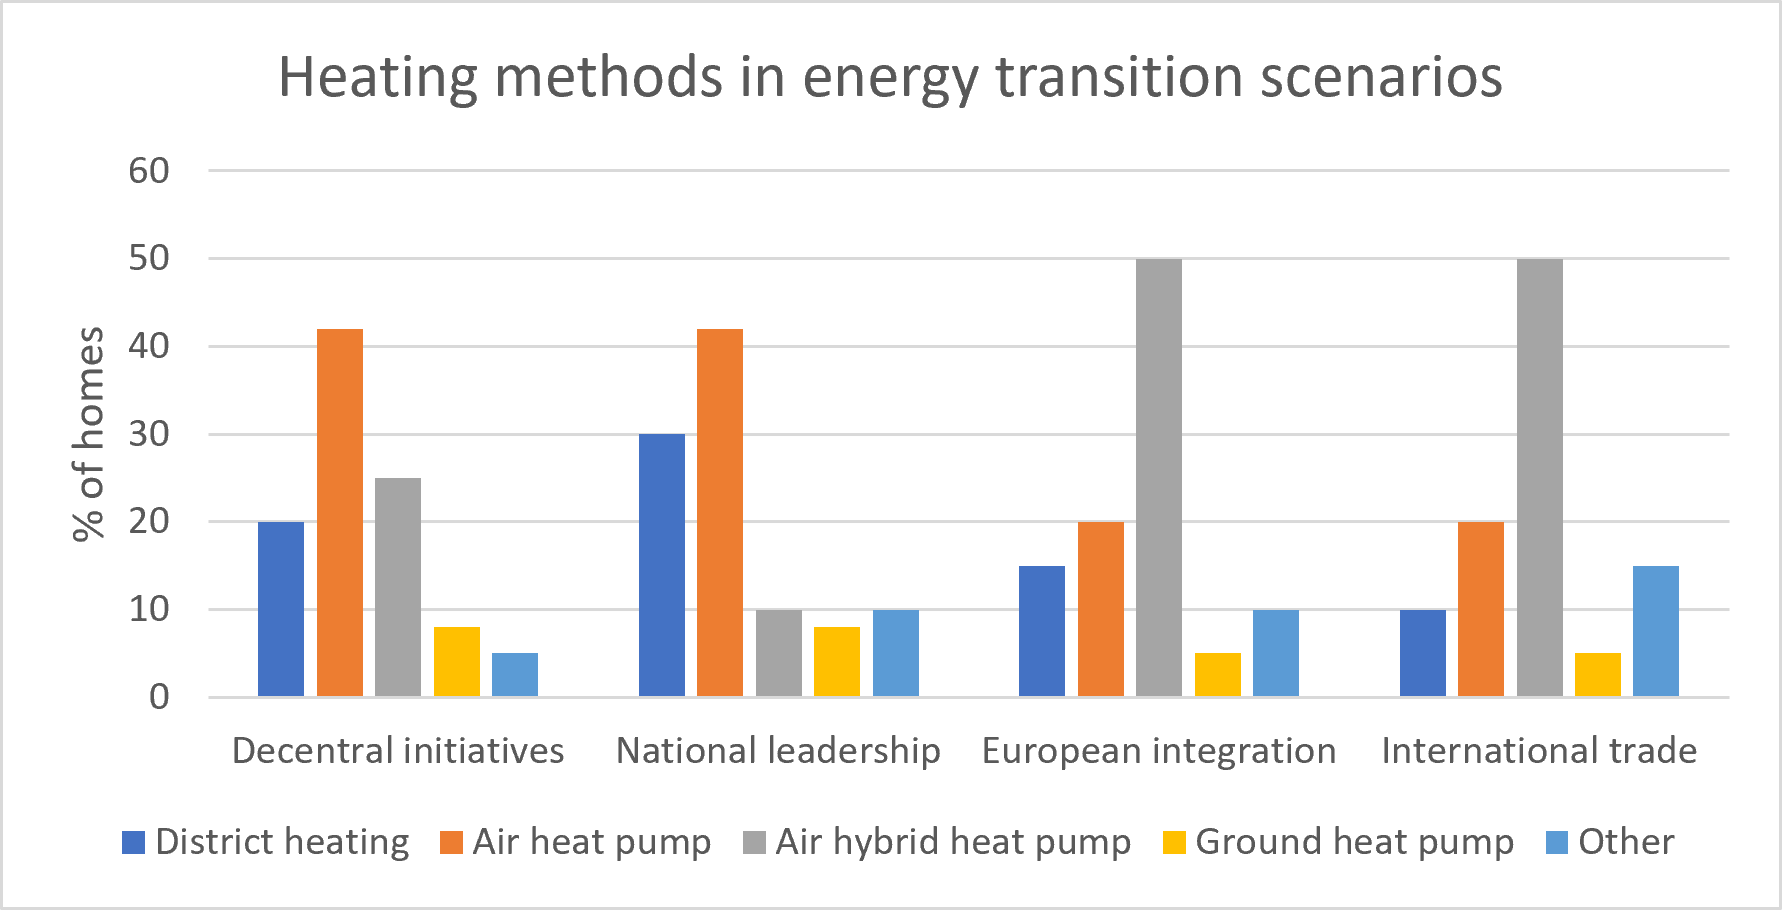
\includegraphics[width=\linewidth]{fig1_heating_scenarios.png}
  \caption{Share of households per heating method in Dutch heat transition
  scenarios by the Dutch association of grid operators \citep{netbeheernederlandHetEnergiesysteemVan2023}.}
  \label{fig:scenarios}
\end{figure}

%% ===========================================================================
\section{Tipping dynamics in the heat transition}
\label{sec:tipping}
%% ===========================================================================

Social-technical tipping points is a concept that aligns to transformative
change in transition studies \cite{meyAnticipatingSociotechnicalTipping2024}. This change only occurs when all
elements in a socio-technical system align, and all system components support the
new system \cite{geelsTechnologicalTransitionsSystem2005}. In this sense, tipping can better not be considered a
single point but a dynamic across the phases of enabling, accelerating, and
stabilizing \cite{sharpeUpwardscalingTippingCascades2021,stadelmann-steffenFrameworkSocialTipping2021,meyAnticipatingSociotechnicalTipping2024}. In recent years, many researchers have categorized and identified numerous
tipping dynamics. \cite{zeppiniThresholdsModelsTechnological2014} start from the perspective of socio-technical transitions. \cite{lentonOperationalisingPositiveTipping2022/ed} expand this to the socio-ecological domain, and \cite{geelsSociotechnicalTransitionPerspective2023} again turn to the transition studies domain and add
feedback loops related to policies and firms to the list. We build on these with
a slightly different dichotomy aimed at distinguishing dynamics in different
domains and identify dynamics which are especially relevant to the residential
heat transition. These are elaborated upon in the following section and
summarized in Table~\ref{tab:dynamics}.

Note, these dynamics do not always lead to system tipping, and aligning to \cite{milkoreitSocialTippingPoints2023}, we do not consider them \emph{tipping models} by themselves.
Instead, we consider them as components or subdomains of the larger
socio-technical system which, when aligned, could trigger larger system tipping.
This also connects to the broader perspective taken in most adoption models
applied to sustainable behavior or technologies, and many of the
micro-foundations as identified by \cite{zeppiniThresholdsModelsTechnological2014}. These models usually
take the perspective of utility maximization in a combination of social,
psychological, technological, and economic factors, going beyond the idea of
single domain-based thresholds such as social critical mass or cost parity.

\begin{table}[htbp]
  \centering
  \caption{System dynamics contributing to tipping behavior.}
  \label{tab:dynamics}
  \footnotesize
  \begin{tabular}{L{2.1cm} L{1.3cm} L{2.6cm} L{3.2cm} L{3.2cm}}
    \toprule
    \textbf{Dynamic} & \textbf{Domain} & \textbf{Tipping phase} &
    \textbf{Example models/theory} & \textbf{Heat transition examples}\\
    \midrule
    Social learning and thresholds & Social &
    Threshold to niche, acceleration when triggered, stabilization to incumbent &
    User and wider publics and technology; information cascades; social
    influence; percolation; network effects &
    Social learning and thresholds in the adoption of new heating technologies\\
    \addlinespace
    Economies of scale & Economic &
    Threshold to niche, stabilization to incumbent &
    Increasing returns &
    District heating requires larger-scale upfront investments than its
    alternatives\\
    \addlinespace
    Economic learning & Economic &
    Threshold to niche, acceleration when triggered, stabilization to incumbent &
    Increasing returns by learning-by-doing and learning-by-using &
    Learning factors in novel technologies such as heat pumps, where more
    granular technologies experience faster learning \cite{wilsonGranularTechnologiesAccelerate2020}\\
    \addlinespace
    Feedback in updating rules, regulations, institutions, and infrastructure &
    Policy & Threshold to niche, stabilization to incumbent &
    Policy--firm feedback \cite{geelsTechnologicalTransitionsSystem2005,edmondsonCoevolutionPolicyMixes2019,mecklingGoverningRenewablesPolicy2019};
    policy--technology--user feedback \cite{geelsSociotechnicalTransitionPerspective2023,kernPolicyMixesSustainability2019};
    policy learning &
    Subsidies to insulation and sustainable heating, proposed ban on natural gas
    boilers, heat transition vision programs, policy involvement in district
    heating, etc.\\
    \addlinespace
    Multi-system interactions, coevolution, and coordination games & System &
    Threshold to niche, stabilization to incumbent &
    Coevolution \cite{vandenberghEvolutionaryTheoriesEnvironmental2000,kauffmanCoevolutionEdgeChaos1991,zeppiniThresholdsModelsTechnological2014}; coordination game \cite{kandoriLearningMutationLong1993,zeppiniThresholdsModelsTechnological2014} &
    Interactions between sustainable heating, electricity and mobility in energy
    prices and grid congestion\\
    \bottomrule
  \end{tabular}
\end{table}

\paragraph{Social learning and thresholds}
provide insights into how behavior shifts by social interaction under different
network structures. Granovetter's threshold model \cite{granovetterThresholdModelsCollective1978} explains how individuals
adopt behavior based on the number of prior adopters. This model is further
extended by incorporating different types of social networks and network
connectivity \cite{wattsSimpleModelGlobal2002}. \citet{wiedermannNetworkbasedMicrofoundationGranovetters2020} show how through micro-interactions
and initial population preconceptions this can lead to saddle-node bifurcations,
or in other words tipping points. The type and level of
detail of social contagion or social learning greatly differs across applications
and models. Where some contagion, such as the spread of information, is
relatively simple, more impactful decisions will result in complex contagion, and
significantly different diffusion outcomes \cite{centolaComplexContagionsWeakness2007}. Although this
variety is broad, the general tendency between all these types of social
contagion, social learning, and social influence \cite{youngInnovationDiffusionHeterogeneous2009}, but also
informational cascades and network effects \cite{zeppiniThresholdsModelsTechnological2014,lentonOperationalisingPositiveTipping2022/ed} is similar. All result in reinforcing feedback loops where initial adopters
lead to an acceleration in more adopters and thus tipping dynamics if these
dynamics result in a changed stable state with a new social norm.

The effect of social learning and thresholds is also well investigated for novel
technologies in the heat transition. Like any innovation, social norms around
novel heating technologies are also improved with increased adoption \cite{raoCriticalReviewHeat2025}. As a new heating system is a relatively big, impactful, and complicated
decision, especially the spreading of information and best practices is important
\cite{broersDecidedDividedEmpirical2019}.

\paragraph{Economies of scale and economic learning}
are primarily driven by increasing returns, in which the value of a technology
increases the more existing users it has \citep{arthurCompetingTechnologiesIncreasing1989}. Forms of increasing
returns are learning-by-doing, learning-by-using, economies of scale, and
network effects. Economies of scale result in a form of threshold, in which an
initial scale is required to become cost competitive with alternative options.
Learning, similarly, results in regime inertia, as incumbent technologies have
further experienced their learning curve, while novel technologies are still
relatively expensive. The extent to which economic learning is also captured with
a threshold is uncertain. While some models look at cost parity, there is ample
evidence that costs are just one of the factors in adoption or investment
decisions.

When looking at the heat transition, sustainable alternatives have vastly
different economic dynamics. District heating systems are well-established
systems, with high upfront investment costs and strong economies of scale. In
other words, they require a large threshold of consumers connected within an area
to be economically viable. This results in non-linear adoption dynamics and
requires alignment between individual households and district heating companies
\citep{herrerasmartinezWhyGoPublic2023}. In contrast, heat pumps are a more direct
replacement by individual homeowners to the current regime of individually owned
gas boilers.

Learning has similar differences between these technologies. District heating
systems have been deployed for over a century, making the current learning factor
for traditional district heating systems low. Only if radical innovation towards
new, small-scale, 5th generation district heating \citep{buffa5thGenerationDistrict2019,yaoStateoftheartAnalysisPerspectives2024} or towards `smart energy systems' \citep{lund4thGenerationDistrict2014} is achieved, or
with substantial subsidies or public investment, new techno-economic triggers and
feedback loops are expected. On the other hand, (hybrid) heat pumps have seen a
rapid increase in deployment in recent years. This has resulted in a rapid
learning curve, where with a doubling in unit capacity the price per unit drops
on average by 27\% \citep{jakobChapter11Heating2020}, while slower learning is expected with a
22\% decrease in investment costs between 2025 and 2050 \citep{europeancommissiondirectorate-generalforenergyBarriersActionDrivers2024}.

From a more theoretical perspective we can distinguish heat pumps as granular
technologies, while district heating systems are `one-of-a-kind' systems. Where
granular technologies generally have a high learning rate \citep{wilsonGranularTechnologiesAccelerate2020},
large infrastructure projects are often characterized by delays and cost overruns
\citep{flyvbjergHowBigThings2023}.

\paragraph{Rules, regulations, institutions, and infrastructure}
are some of the core concepts in transition studies, often highlighting the
inertia, or resistance to change, of existing systems and dominant regimes \citep{geelsTypologySociotechnicalTransition2007,geelsTechnologicalTransitionsSystem2005,verbongOngoingEnergyTransition2007}. From the tipping point
perspective, \citet{geelsSociotechnicalTransitionPerspective2023} define potential reinforcing feedback loops
in this area as well: when firms, users and the wider public start accepting and
embracing a novel, sustainable technology, this results in increased policy
support, rapidly shifting regulations, subsidies, and required infrastructural
projects.

The policy domain can also not be underestimated in the residential heat
transition. In the Netherlands, policymakers take a central, orchestrating, and
directing role \citep{loomansExploringTradeoffsDecisionsupport2024,herrerasmartinezMunicipalitiesKeyActors2022,hoppeLocalGovernmentsSupporting2015}, especially aimed at developing collective infrastructure,
rules, and regulations, and at providing subsidies for sustainable heating and
energy efficiency technologies. However, evidence of the theoretical feedback
loops is less apparent in the current phase. Policymakers are driven by climate
goals, while the public perception towards sustainable heating is mixed
\citep{beauchampetEnergyCitizenshipNetherlands2021,herrerasmartinezMunicipalitiesKeyActors2022,jansmaKissingNaturalGas2020,voetenEnergyTransitionSupport2025}.

\paragraph{Co-evolution and coordination games}
originate from evolutionary economics and game theory. When thinking of
socio-technical systems from an evolutionary perspective, the notion of
coevolution makes sense, as these systems are shaped by all stakeholders
involved, which coevolve towards a stable regime. In fact, nearly all evolution
can be considered coevolution \citep{vandenberghEvolutionaryTheoriesEnvironmental2000}. From a tipping
perspective, coevolution is important as tipping dynamics in one system or system
component can trigger dynamics in another. In the same way, closely coevolved
systems can be rigid as all system components need to change to destabilize the
system. Coevolution can be considered across different scales and system levels.
Where multiple actors within a socio-technical system adapting to each other is
seen as coevolution, multi-system interactions can also be considered coevolution
on a higher scale.

Apparent multi-system interactions in the residential heat transition are the
connection to the mobility and sustainable energy generation transitions. All are
vital components of the broader energy transition, and meet on shared
infrastructure such as electricity grids and through sector coupling \citep{rinaldiDecarbonisingHeatOptimal2021}. Coevolution occurs in the interaction between stakeholders, especially
in the interaction between homeowners, landlords, and social housing associations.
For example, social housing associations owning a large share of dwellings in an
area are often seen as potential launching customers for district heating systems
as they can reach the required scale in number of dwellings more easily. This
enables homeowners and smaller landlords to profit from this new infrastructure
as well. In another case, rapid adoption of heat pumps by environmentally minded
homeowners in an area could diminish the business case and social capital for
district heating systems, creating a lock-in towards individual heating systems.
Note, in these examples multi-system interactions coalign with economies of scale
or increasing returns, connecting a tipping trigger to an acceleration dynamic.

%% ===========================================================================
\section{Modelling transition dynamics}
%% ===========================================================================

The transition dynamics described in the section above have been investigated in
a scenario study using an agent-based model. Agent-based modelling is the most
suitable method to explore such behavior, because of its focus on individual
heterogeneous agents influencing each other and the environment, and ample
examples exist of ABMs simulating the above-mentioned dynamics individually.
Furthermore, ABMs have been extensively used to model energy transition dynamics
\citep{hansenAgentbasedModellingSociotechnical2019b,liReviewSociotechnicalEnergy2015a}, including individual adoption and
diffusion \citep{mogliaReviewAgentBasedModelling2017,duModellingEnergyefficientRenovation2022}, and infrastructure decisions
\citep{chappinAgentbasedModellingEnergy2010}.

In this section we build upon literature on adoption models on the residential
heat transition, although this domain has been relatively underexplored in the
modelling community compared to the adoption of electric vehicles (EV) and PV
\citep{hansenAgentbasedModellingSociotechnical2019b}. The residential heat transition differs from EV and PV
adoption in two important ways. First, there are many more competing alternatives
in the heat transition. Where PV adoption is a yes-or-no decision, sustainable
heating requires careful consideration between heat pumps, hybrid heat pumps, and
district heating solutions. This competition is often lacking within adoption
models \citep{hesselinkAdoptionEnergyEfficient2019}. Second, these choices strongly depend on
external and contextual factors (e.g.\ the construction of a district heating grid
in my neighborhood), are highly influenced by dwelling properties, and have a
significant impact on daily life as many solutions require extensive home
renovations. The literature that does exist in this area mostly focusses on heat
pump adoption and energy efficiency measures such as insulation and home
renovation \citep{raoCriticalReviewHeat2025,hansenFullEnergySystem2019}. These models typically focus
on homeowners making individual investment decisions, although notable exceptions
exist aimed at collective decisions in homeowner associations \citep{navaguerreroAgentBasedModelingThermal2019} and thermal energy communities \citep{navaguerreroAgentBasedModelingThermal2019,fouladvandFormationContinuationThermal2020} and district heating systems \citep{buschScalingLocalEnergy2017,akhatovaAgentBasedModellingUrban2022}.

\subsection{Model description}

The model is an agent-based representation of the Dutch energy system including
actors who make investment decisions. In the following section the model will be
outlined; more detail can be found in Appendix~\ref{app:model}.

The model has annual timesteps, where every year the adoption and expansion
decisions as shown in Figure~\ref{fig:flowchart} are assessed per agent. The
model includes several types of actors: households who are homeowners, social
housing associations, landlords, a grid operator, and a district heating company
(see Table~\ref{tab:agents}). Next to these actors, neighborhoods are used as
spatial demarcation at which households are aggregated; this enables electricity
grid and district heating operators to make decisions at a collective level,
which aligns to current heat transition policies and investment planning of grid
operators and district heating companies.

With these actors we can model all the above-mentioned tipping dynamics: social
learning amongst homeowners, economic learning based on adoption rates, economic
thresholds by business cases for district heating grids by the district heating
companies, and multi-system interaction and coevolution by grid operators,
district heating companies, homeowners, housing associations and landlords.
Lastly, the policy component is introduced in the scenario analysis by means of
rules, regulations, and subsidies. We choose not to model this feedback loop
endogenously as it is highly uncertain and not quantitatively researched for the
Dutch heat transition.

Each of the actors is further described in the following section.

\begin{figure}[htbp]
  \centering
  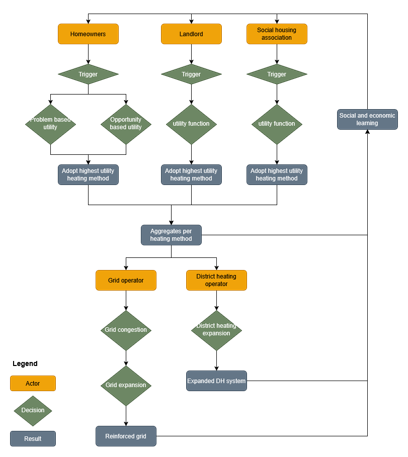
\includegraphics[width=0.9\linewidth]{fig2_model_flowchart.png}
  \caption{Flow chart of model dynamics.}
  \label{fig:flowchart}
\end{figure}

\begin{table}[htbp]
  \centering
  \caption{Description of agent populations in the model.}
  \label{tab:agents}
  \footnotesize
  \begin{tabular}{L{2.4cm} L{2.0cm} L{8.4cm}}
    \toprule
    \textbf{Agent populations} & \textbf{Population size} &
    \textbf{Agent behavior}\\
    \midrule
    Dwellings & $\sim$8 million &
    Each single dwelling in the Netherlands is simulated. Its characteristics are
    determined from neighborhood statistics, and they are attributed to
    decision-making agents based on their ownership.\\
    \addlinespace
    Homeowners & $\sim$4.6 million &
    Most dwellings in the Netherlands are privately owned. Each dwelling with a
    private homeowner is assigned a household which owns the dwelling. On an
    annual basis each household makes an adoption decision on heating source and
    insulation based on a utility function combining costs with attitude and
    social norms, and the possibility of each option.\\
    \addlinespace
    Social housing association & 1 &
    The social housing company has the goal to get a climate-neutral housing stock
    by 2050. To do this they can invest in insulation and sustainable heating
    methods. They have the power to shift a large percentage of households in a
    specific area towards a certain heating method, making them a valuable partner
    for the infrastructure and policy actors. They assess groups of households on
    a neighborhood level, making annual adoption decisions for all houses they own
    within an entire neighborhood at once.\\
    \addlinespace
    Landlords & $\sim$1.2 million &
    All dwellings owned by landlords are assigned a landlord. Like homeowners,
    landlords make annual adoption decisions. However, they are primarily focused
    on economic revenue instead of social and psychological norms and values.\\
    \addlinespace
    Grid operator & 1 &
    The grid operator makes choices on where to reinforce the electricity grid. If
    the grid is reinforced this enables more households to adopt electric heating
    such as heat pumps.\\
    \addlinespace
    District heating company & 1 &
    District heating companies make investment decisions on where to build
    district heating grids, enabling district heating as a heating method for
    households. They have three potential strategies for expansion: (1) based on
    policy plans; (2) based on the number of interested households; and (3) based
    on a combination of these measures.\\
    \bottomrule
  \end{tabular}
\end{table}

\subsubsection{Dwellings}

In the model we simulate all households in the Netherlands (over 8 million) with
their individual, heterogeneous household characteristics. We use individual
building data on construction year, size, and type of dwelling from the Dutch
building administration \citep{kadasterDatasetBasisregistratieAdressen2022}. Based on neighborhood characteristics
each building is given a current heating method, in-house heat distribution
system, and insulation level. All dwellings are owned by either a homeowner, the
social housing association, or landlords.

\paragraph{Cost calculations and economic learning}
The costs are calculated using the Equivalent Annual Costs (EAC) for a fair
comparison between heating methods with different investment costs, operational
costs, and lifetimes \citep{hastingsFinancialMethods2021}. Furthermore, the costs depend on the
required insulation levels and in-house heat distribution system. For all-electric
heat pumps, low-temperature in-house heat distribution and a high level of
insulation is required for efficient operation. If these are not yet installed,
additional costs are added to the investment costs. This does of course lead to
reduced heat demand, which decreases operational costs. Annual heat demand,
electricity demand, and costs for insulation are based on dwelling type,
construction year, and energy label, with data from VestaMAIS, a model aimed at
the Dutch built environment energy transition \citep{pblHetVestaMAIS2017,vandermolenFunctioneelOntwerpVesta2021}.

As insulation and heat distribution are key components in the cost calculation, we
need to consider home renovations as well. The building stock is under continuous
development. Homes are renovated approximately once every 25 years, where
insulation and heat distribution systems are upgraded independently from heating
system adoption decisions. These measures are considered exogenous to the model,
but as they affect the heating method adoption decision, their effects are
included by randomly improving insulation levels and heat distribution systems in
households every 25 years.

Costs of heating methods for each dwelling are updated each time the adoption
function for the owner of that dwelling is triggered. After all owners made their
adoption decision, national cost assumptions are updated using the learning curve
formula (Wright's law) based on the initially installed units, added units,
initial costs and learning rate. As described in Section~\ref{sec:tipping}, the
learning rate differs per technology. A more detailed description of the EAC and
economic learning calculations can be found in Appendix~\ref{app:cost}.

Two further elements shape the cost signal over time. First, equipment does not fail deterministically: each installed system's end-of-life age is drawn from a normal distribution around its nominal lifetime ($\pm 3$ years), so that replacements are spread out. Second, gas and electricity retail prices evolve along an assumed annual growth path, kept constant in
the baseline scenario and varied as a coupled low/high bracket in the sensitivity analysis (Section~\ref{sec:calibration}), with bounds taken from the Dutch national Climate and Energy Outlook \citep{pbl_kev_2025}. 

\subsubsection{Homeowners (households)}

Most dwellings in the Netherlands (57\%) are privately owned. This also means that investment-related decisions are made by the primary residents. All 4.6 million privately-owned dwellings are represented in the model as household agents, who make annual adoption decisions on heating methods. These households combine the technical characteristics of the dwelling with their social network, attitude, and financial preferences in an adoption function.

\paragraph{Adoption function}
Literature on household adoption models of sustainable heating methods is varied. The most used framework is the theory of planned behavior \citep{sophaAdoptionDiffusionHeating2013,okurAdoptionRenewableHeating2024,sophaExploringPolicyOptions2011}, however, many other models have a
non-theory-based utility function \citep{raoCriticalReviewHeat2025}.

An important distinction between models is the structure of the decision-making
process. Most papers using utility functions integrate this in a single-stage
decision; once the utility threshold is reached, the decision-maker will adopt
\citep[e.g.][]{snapeWillDomesticConsumers2015,melesAdoptionRenewableHome2022}. Multi-stage decision-making models acknowledge the complexity of making home renovation and heating method decisions. \citet{hecherTriggerMattersDecisionmaking2017} identify the trigger, selection, and decision stages. In this they differentiate between triggers, which are problem-based, opportunity-based, or a new building. A problem-based trigger occurs when the current heating system breaks down, while an opportunity-based trigger comes from
a subsidy program or planned renovation. Problem-triggered adoption decisions often result in simple substitution without shifting heating methods, while
opportunity-based triggers often result in shifts towards more sustainable heating
methods \citep{broersDecidedDividedEmpirical2019}. Thus, homeowners should be reached and triggered before their current heating system breaks down.

Commonly used factors in models representing these decisions are economic utility,  attitude and norms towards a technology and peer network effects and social learning.
Economic utility is usually included in the form of investment costs, discounted annual heating costs, or payback times \citep[e.g.][]{snapeWillDomesticConsumers2015,melesAdoptionRenewableHome2022,michelsenMotivationalFactorsInfluencing2013}. This economic factor often disperses into extensive building modelling of a heterogeneous dwelling stock with different costs and requirements in home renovation and heating methods based on the building type, construction year and surface area
\citep[e.g.][]{leeAnalysisUKPolicies2014}. Attitude or personal norm towards the different heating methods are usually aimed at sustainability, ease of use, or technological novelty \citep[e.g.][]{snapeWillDomesticConsumers2015,melesAdoptionRenewableHome2022}.
Network effects and social learning are often included by focusing on the number of adopters in a network, or with more extensive social interactions and peer network modelling \citep[e.g.][]{snapeWillDomesticConsumers2015,navaguerreroAgentBasedModelingThermal2019,melesAdoptionRenewableHome2022}.

As the goal of this paper is to identify tipping points, we opt for a
relatively simple adoption function, based on the theory of planned behavior as used by \citet{okurAdoptionRenewableHeating2024}. 
% TODO We extend this framework in three ways. Based on \citet{hecherTriggerMattersDecisionmaking2017} we add different triggers, in which we consider the `new house' trigger as a type of opportunity trigger. Now, if a household is triggered by either an opportunity or a problem, the household compares alternatives based on the highest-ranking utility. This utility is calculated by using the theory of
% planned behavior as applied by \citet{okurAdoptionRenewableHeating2024}.

TPB consists of five components. First, the attitude towards each heating method
is set during agent initialization with values ranging between 0 and 1. This value
remains constant throughout the simulation. Second, the subjective norm towards
each heating method reflects social influence exerted by the agent's peer network.
It is recomputed every year as the share of network peers currently using that
method, amplified by a technology \emph{salience} factor that captures how socially
visible the method is (Equation~\ref{eq:sn}, with $s_{hm}$ the peer adoption share
and $\sigma_{hm}$ the salience, capped at one). Salience follows an S-curve in the
method's population share (Equation~\ref{eq:salience} in Appendix~\ref{app:model}):
a novelty term makes emerging, low-share methods more salient, while a momentum term
raises salience for methods whose share is growing. Social influence is therefore
self-reinforcing as adoption of a method grows, its salience, and hence its
subjective norm rise, feeding further adoption, which is the mechanism through
which social tipping can arise. The strength of this channel is scaled per
technology by a social-learning rate, which is varied in the scenario analysis.

\begin{equation}\label{eq:sn}
  SN_{hm} = \min\!\left(1,\; s_{hm}\cdot\left(1 + \sigma_{hm}\right)\right)
\end{equation}

Next, the perceived behavioral control is calculated (see Equation~\ref{eq:pbc}) by
combining the affordability and effort of each heating method. Affordability is
one minus the normalized equivalent annual cost (EAC) of the method; the EAC ensures
a fair comparison between methods with different investment costs, operational costs
and lifetimes, and includes required investments for in-house heat distribution and
insulation. To preserve the relative cost differences a household actually faces, the
EAC is normalized on a single \emph{logarithmic} scale that covers all methods and
dwellings in that year (Section~\ref{sec:calibration}). Effort is a fixed value
between 0 and 1 assigned to each method, differing between keeping the current method
and switching to an alternative (an alternative that requires a low-temperature
retrofit carries the highest effort). The trigger type (problem-based versus
opportunity-based) governs whether and when a household evaluates its options rather
than entering the control term directly.

\begin{equation}\label{eq:pbc}
  PBC_{hm} = \frac{\left(1 - \widehat{EAC}_{hm,n}\right)\cdot w_{costs}
    + \left(1 - Effort_{hm,n}\right)\cdot w_{effort}}
    {w_{costs} + w_{effort}}
\end{equation}

The intention for each heating method is calculated using the standard TPB
implementation of the combined value of attitude, subjective norms, and PBC
multiplied by their weights (Equation~\ref{eq:intention}). Similarly, utility is
calculated by the sum of intention and PBC multiplied by their weights
(Equation~\ref{eq:utility}). Lastly, the utilities of all options are filtered to
exclude non-available options (e.g.\ no district heating if there is no heating
grid in the neighborhood), and from the filtered set the option with the highest
utility is selected and adopted (Equation~\ref{eq:argmax}).

\begin{equation}\label{eq:intention}
  Intention_{hm} = \frac{Att_{hm,n}\cdot w_{Att}
    + SN_{hm,n}\cdot w_{SN}
    + PBC_{hm,n}\cdot w_{PBC}}
    {w_{Att} + w_{SN} + w_{PBC}}
\end{equation}

\begin{equation}\label{eq:utility}
  Utility_{hm} = \frac{Intention_{hm,n}\cdot w_{intention}
    + PBC_{hm,n}\cdot w_{PBC}}
    {w_{intention} + w_{PBC}}
\end{equation}

\begin{equation}\label{eq:argmax}
  \text{Selected heating method} = \argmax_{hm \in HM} U_{hm}
\end{equation}

Note, this is a simplified adoption model. Many more elaborate approaches and
different frameworks exist; however, in this study the focus is on evaluating
effects of interactions with different stakeholders instead of further detailing
the adoption process of individual households.

\paragraph{Homeowner initialization}
This agent is initiated with all relevant parameters for the adoption function
stated in the previous section. The attitude per heating method and social network
are initialized. The initial distribution of attitude values is calculated as the
difference between the sustainability score given to each heating method and a
sustainability attitude set per household based on a normal distribution with
values from \citet{okurAdoptionRenewableHeating2024} and \citet{broersDecidedDividedEmpirical2019}. Currently, Dutch households have
a positive attitude towards sustainable heating methods. However, their subjective
norms are neutral and their perceived behavioral control is low \citep{okurAdoptionRenewableHeating2024}. To reflect any correlation between these parameters, Cholesky decomposition
is used for all parameter values attributed during the model initialization phase
\citep{edlinCorrelatedParametersCholesky2015}. After the initial intention is calculated, small-world
networks are initialized for all homeowners, where they are most likely to connect
to homeowners with a similar sustainability attitude within their municipality,
while also having some random connections throughout the population.

\subsubsection{Social housing associations}

Social housing associations can have a large impact on the optimal heating system
in a neighborhood. As, depending on the neighborhood, they can own up to 90\% of
the dwellings, their decision also has a large impact on individual homeowners.
Furthermore, it enables district heating companies and grid operators to get into
strategic decisions and plan on when to expand where. For example, neighborhoods
with high shares of social housing are seen as most promising by district heating
operators, as it reduces the risk of low connection percentages when the housing
association connects all its houses to the district heating system. This makes
them a more powerful actor than individual homeowners in the same neighborhood.

Although the additional power brings an interesting dimension to actor
interactions, actual adoption of sustainable technologies by housing associations
has been slow \citep{filippidouAreWeMoving2017}. Adoption is characterized by a complex
interplay between social housing association, tenants, and local governments.
Initial ambitious goals of housing associations have been lowered due to issues
with financial feasibility and a lack of trust from tenants \citep{hoppeAdoptionInnovativeEnergy2012}. However,
as no quantitative data on these dynamics exists, we consider social housing
associations as rational actors in heating system adoption decisions. They can have
different strategies which will be evaluated in the scenario analysis. The first
strategy is a simple problem-based replacement when a system breaks down based on
the lowest annual costs per dwelling (see Appendix~\ref{app:cost} for the exact
equation). Although the housing associations typically only pay the investment
costs, and the tenant pays for the gas, electricity or heat costs, we do consider
the EAC as we assume that housing associations have an incentive to reduce annual
costs as this can raise their rental tariffs or eventual selling prices \citep{chegutEnergyEfficiencyEconomic2016}. The second is an opportunity-based approach which aligns to current
policy plans of heating systems per neighborhood as determined in the heat
transition visions policy documents \citep{molenOverzichtTransitievisiesWarmte2023}. This approach aligns to
policy advice on accelerating the heat transition \citep{vringerSavingEnergyNot2016}, and it
could enable more district heating due to the role of launching customer for these
associations.

\subsubsection{Landlords}

Landlords in themselves are a very heterogeneous group, ranging from large real
estate investment companies (or institutional or corporate landlords) with
thousands of dwellings to private landlords who own one or several properties and
rent them out personally \citep{lennartzParticuliereVerhuurdersOp2019}. In this, especially private
landlords have a wide variety of decision-making dynamics in home renovations and
heating system adoption, including values, beliefs, norms and routines next to
economic factors \citep{marzEconomicsUnderstandingDecisionmaking2018,miuPrivateLandlordsEnergy2020,lennartzParticuliereVerhuurdersOp2019}. This
has resulted in slow adoption of energy efficiency and sustainability measures in
privately rented homes \citep{hopeAttitudesBehavioursPrivate2014}. However, like social housing
associations, not enough data exists to model this in full detail, as not even the
distribution between the different types of landlords per region is known.
Therefore, also like the social housing association, we consider landlords to be
rational actors who only invest in dwellings if they can replace the current
system by a cheaper one (see Appendix~\ref{app:cost} for the exact equation).
Again, although the landlords typically only pay the investment costs, and the
tenant pays for the gas, electricity or heat costs, we do consider the EAC as we
assume that landlords have an incentive to reduce annual costs as this can raise
their rental tariffs or selling prices. Landlords do not have any additional
strategies.

\subsubsection{District heating operator}

District heating operators try to expand their district heating system. In the 
model they make the decision to expand the district heating network per
neighborhood on an annual basis. Like social housing associations, they do this
based on their growth strategy. They can have two strategies: either they follow
current policy plans, or they expand based on their expected business case. The
first strategy simulates a top-down policy push, where the district heating system
is installed independently of demand. The second is demand-driven, where the
district heating operator acts if the number of households interested in
connecting, and with that the heat demand per hectare, crosses the positive
business case threshold (600 GJ/ha) and it will develop a heating grid. This is
calculated by aggregating the heat demand of the dwellings for which district
heating is the preferred heating method. In terms of tipping points, this
resembles a threshold caused by increasing returns. The threshold represents about
50--80\% of the dwellings in an area. Once the threshold is crossed and the
district heating system is built, it becomes possible for other households to
connect to the system as well. Again, for modelling purposes this is a simplified
approach to actual district heating expansion. In reality public acceptance,
strong support policies, institutions such as regulators, and business models are
all essential in expanding district heating systems \citep{bertelsenImplementingLargescaleHeating2021,saliteAssessingAdoptionSustainable2024,onencanSocialAcceptanceDistrict2024}.

\subsubsection{Electricity grid operator}

In the model, grid operators manage and expand current grid congestion. After the
households, social housing associations and district heating grid operators have
made their adoption and investment decisions, the grid operator reacts by
calculating the new peak electricity demand per neighborhood. If the peak
electricity demand exceeds the current capacity, the grid operator reacts by
reinforcing the grid in this neighborhood. Other big new loads such as electric
vehicles are included with a simplistic S-shaped adoption curve, as they are not
the core of the paper but have significant impact on grids.

From a tipping perspective, the grid can become a threshold to electric heat pump
adoption, and thus shape pathways. Alleviating this bottleneck can enable
reinforcing learning feedback loops. Too slow action can result in investment
decisions in district heating, and thus path dependency and lock-ins.


\section{Analysis design}
\label{sec:design}
%% ===========================================================================
The model is used to establish how the tipping mechanisms of
Section~\ref{sec:tipping} influence transition pathways. Although these dynamics
are well established in transition literature, data on them is scarce. 
This makes calibration and validation especially hard. Furthermore, calibrating to
current data leads to an extrapolation of current trends, while we are interested 
precisely in the deviations from those trends that non-linear dynamics produce.
Therefore, we have setup an exploratory analysis design combining established components,
based on analysis types as noted by \citet{leeComplexitiesAgentBasedModeling2015}.
Starting with history matching to create an ensemble of plausible decision weights 
\citep{beven_future_2006}. Then ranking the influence the uncertain parameters using 
Morris elementary effects, and quantifying those using Latin-hypercube sampling. 

We use this ensemble and sensitivities in the scenario analysis, which is focussed 
on examining tipping or non-linear dynamics. For every tipping mechanism, the 
governing parameters are varied to bound its influence, its reinforcing loop is 
disabled to establish causal necessity, and where a threshold is expected its driver 
is swept continuously to locate it. Discrete policy measures enter as levers within 
the mechanism on which they act. Also, we give in detail insights in how some of 
these tipping dynamics can be triggered by specific agent groups. 

The full design is summarized in the following five steps and 
Figure~\ref{fig:method_flowchart}, each step is explained in more detail in this section.

\begin{enumerate}\itemsep2pt \parskip0pt
  \item \textbf{Calibrate plausible decision weights.} A sample of candidate weight sets is
        scored against historic data and the plausible ones retained as an ensemble,
        using the Generalized Likelihood Uncertainty Estimation (GLUE) framework.
  \item \textbf{Rank uncertain parameters.} Morris elementary effects establish which of
        the process and techno-economic parameters most influence the 2050 mix.
  \item \textbf{Quantify key uncertain parameters;} Those that rank highest are sampled by
        Latin-hypercube design, and their direction and magnitude are quantified using standardized
        regression coefficients.
  \item \textbf{Run  pathways and experiments.} The retained ensemble is
        carried across the scenario matrix at national scale, with knock-out runs and driver
        sweeps to isolate each mechanism.
  \item \textbf{Report in separate household segments,} such as adopter and ownership segments, to show
        which groups drive each dynamic.
\end{enumerate}

\begin{figure}[htbp]
  \centering
  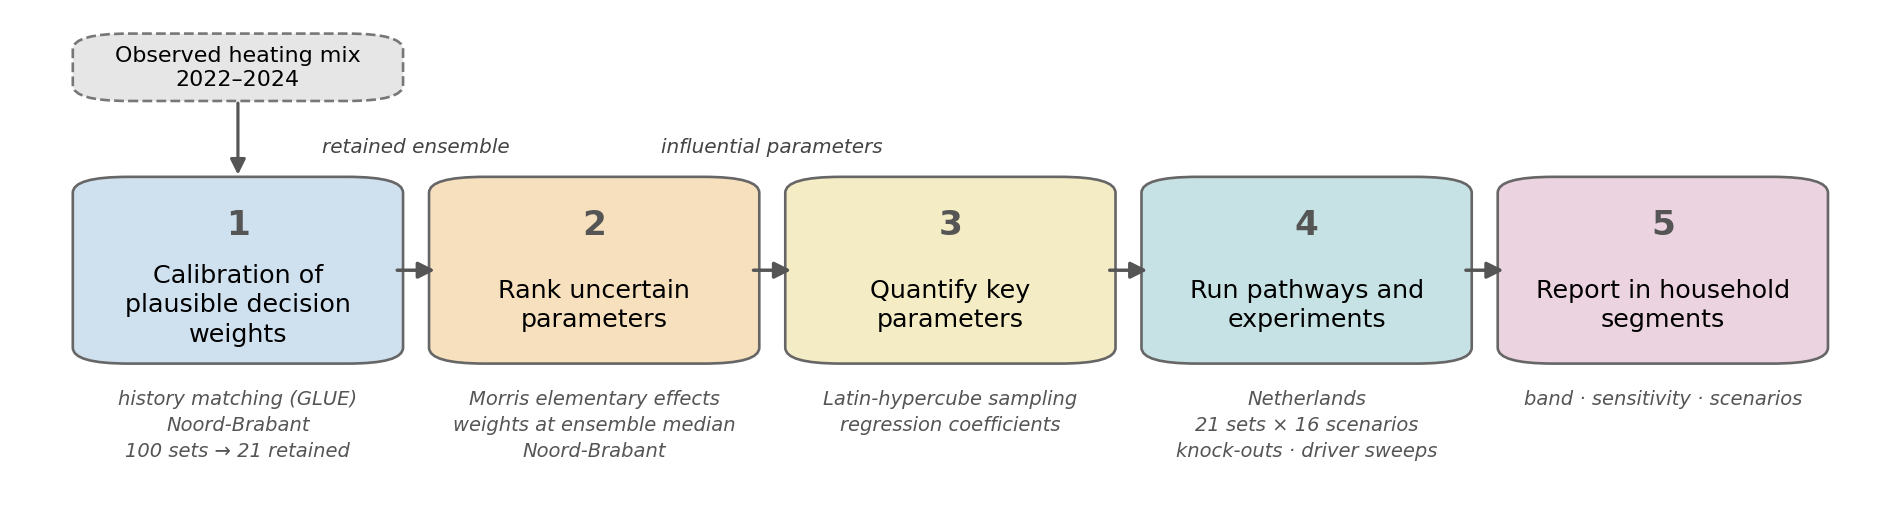
\includegraphics[width=1\linewidth]{figures/fig_method_flowchart.png}
  \caption{The five-step analysis design. Calibration and parameter screening are carried out
    on the calibration region (Noord-Brabant); the scenario pathways and mechanism experiments
    are run for the full Netherlands.}
  \label{fig:method_flowchart}
\end{figure}

%% ---------------------------------------------------------------------------
\subsection{Dealing with uncertainty}
\label{sec:uncertainty}
We distinguish the standard categories, stochastic, parametric, and structural uncertainty. 
\emph{Stochastic} variability arises from the model's random draws, which include: 
household attitudes, network formation, heating method failure ages, and
randomization in the adoption function. This stochastic variability is tested by calculating 
the required number of replications per analysis (see Appendix~\ref{app:replication}). For the 
calibration, morris and national scenario runs this is just one replication, for the LHS this is eight.
So few replications are required because the stochastic variability occurs on individual household
level, for which there are over 8 million in the national analysis, averaging out this uncertainty 
within a single replication. Even though one is the minimum, the national scenarios are run with two
replications.

\emph{Structural} uncertainty concerns the form of the model itself: whether the
theory of planned behavior is the right account of the adoption decision, or the S-curve the
right description of social visibility. This uncertainty is not quantified, but addressed 
through the model's grounding in the literature (Section~\ref{sec:model}) and its verification 
(Section~\ref{sec:verification}).

\emph{Parametric} uncertainty concerns the numerical assumptions of the model. 
Most parametric uncertainty occurs from process assumptions (e.g. salience factor),
techno-economic assumptions (e.g. energy prices) and weights in the decision-making framework. 
The process and techno-economic parameters are analyzed in a sensitivity analysis, while the 
decision weights are filtered plausible weight-sets based on historic matching, as described in the next section.

%% ---------------------------------------------------------------------------
\subsection{Calibrating to plausible decision weights}
\label{sec:calibrating}
Ideally, a model would be calibrated to the data that underlie these assumptions. However, the 
only consistent data set on the adoption of heating methods in the Netherlands spans just three
years (2022-2024). This short observation window cannot uniquely identify the decision weights:
many combinations reproduce recent adoption equally well. Rather than forcing a best-fit and risking
overfitting, we use history matching within the Generalized Likelihood Uncertainty Estimation
(GLUE) framework \citep{beven_future_2006}. Each weight is bounded by a plausible range around the
values reported by \citet{okurAdoptionRenewableHeating2024}. A Latin-hypercube sample of 100 weight
sets is drawn across this space and used as simulation input. Every set whose simulated 2022--2024 
change in the provincial heating mix falls within a tolerance of the observed change is retained, 
the rest is discarded. To keep the sampling behaviorally interpretable, we vary normalized shares 
within each stage of the decision function rather than raw weights, which reduces the space to
four free parameters. The retained sets constitute a plausibility ensemble that is carried into 
the scenario analysis, so that pathways are reported as a band across behaviorally plausible
preferences rather than a single fitted line. In the sensitivity analysis, the median weight-set 
was used. The ensemble is itself a result and is reported as such in Section~\ref{sec:res-ensemble}.

Calibration is carried out on the province of Noord-Brabant over 2022--2024, the most recent
window for which the Dutch statistics office reports a methodologically consistent
per-neighborhood heating-mix series. Each weight set is scored by the mean absolute deviation
of its simulated 2023 and 2024 mixes from the observed mixes, taken across the three
technologies that move materially over the window (natural gas boilers, hybrid and electric heat pumps). 

This calibration is done with two iteration per weights set. This is already more than required as 
the standard deviation between iterations is much smaller than the set tolerance (0.028 compared to 
2 percentage points). See Appendix~\ref{app:replication} for more detail).

%% ---------------------------------------------------------------------------
\subsection{Sensitivity to process and techno-economic parameters}
\label{sec:sensitivity}
To rank the most relevant process and techno-economic assumptions made in the 
model (step 2), the Morris elementary effect design 
\citep{morris_factorial_1991, campolongoEffectiveScreeningDesign2007} was used. As the model 
contains more uncertain assumptions than can be varied jointly, the Morris design is used to 
rank these parameters and taking only the most relevant for a full sensitivity analysis. 
Morris works by moving one factor at a time along a small number of random trajectories through 
the parameter space. Each step changes a single factor and records the resulting change in the
outcome, an elementary effect, and the mean absolute elementary effect, $\mu^{*}$, ranks the 
factors by influence. The standard deviation of the elementary effects, $\sigma$, indicates 
whether a factor acts on its own or only in combination with others. For this analysis the 
decision weights are held constant at the median of the ensemble, and the elementary effects 
are compared on the full 2050 technology mix. 

The highest-ranked parameters are then quantified by Latin-hypercube sampling 
\citep{mckayComparisonThreeMethods1979} over those parameters alone (step 3). In this we use 
standardised regression coefficients giving the direction and relative magnitude of each 
effect, and the coefficient of determination indicating how much of the variation in each 
technology's 2050 share they jointly explain \citep{saltelli_global_2008}. 

Two special cases of parameters are treated separately. Three of the nine parameters govern 
the salience factor of the decision-making algorithm. This mechanism specifically affects the 
peer-adoption share and, with that, the subjective norm. So in weight sets from the ensemble in
which the subjective norm weight is low, these parameters may seem like they have little influence, 
whereas they would have more influence in sets with a large weight for subjective norms. For this 
reason, the analysis is repeated across several weight sets. Second, gas and electricity prices 
are treated as a coupled factor. The range of these are taken by extrapolating prices from the high 
and low bounds in Dutch policy scenarios \citep{pbl_kev_2025}. These are coupled in high and low 
combined gas and electricity prices, as in the current electricity system natural gas prices strongly 
affect electricity prices. Similarly to the calibration set-up, the Morris analysis is run on the 
province of Noord-Brabant because it requires several hundred additional model evaluations and 
concerns parameter influence rather than national quantities.

%% ---------------------------------------------------------------------------
\subsection{Scenario pathways and mechanism experiments}
\label{sec:mechdesign}
The analysis is organized around the tipping mechanisms identified in
Section~\ref{sec:tipping}. In a second stage, policy measures are introduced to investigate their
effects on these mechanisms. Table~\ref{tab:scenarios} states the resulting
setup: each row gives one mechanism's continuous parameters, its discrete levers, and the loop
experiments run on it. 

Two methods are used to identify tipping dynamics (step 4), ablation scenarios, and driver sweeps. 
An \emph{ablation}, or knock-out, scenario tests what happens when one reinforcing loop is disabled
while everything else is held identical, similar to an one-at-a-time (OAT) analysis {tenbroekeWhichSensitivityAnalysis2016}. 
The difference between the intact and the knocked-out scenario is the causal contribution of that loop. 
A \emph{driver sweep} varies a single driver continuously, so that the threshold at which the pathway 
changes shape can be located. 

The general exploration (row~0 of Table~\ref{tab:scenarios}) is run first and deliberately
precedes the isolation of any single mechanism. It establishes which features of the pathway are
robust across the full space of plausible weights and process and techno-economic assumptions,
and which are not. Only outcomes that vary within that space are candidates for mechanism-level
explanation; the mechanism sections that follow then attribute the variation to specific loops.

Pathways are assessed as the share of dwellings per heating method over 2024--2050, with
attention to the moments and rates of acceleration or deceleration that indicate a tipping point,
and are reported as ensemble bands rather than single lines. Because the decision weights and the
process and techno-economic parameters are separate kinds of uncertainty, results are reported separately: 
the preference band, the parameter sensitivity, and the exogenous price and policy
scenarios. Results are also reported per household segment to show which groups drive
each dynamic. A policy-oriented synthesis of the levers across all mechanisms closes the results.

\begin{table}[htbp]
  \centering
  \caption{Experimental design by tipping mechanism. Each row states the full design for one
  mechanism: the continuous parameters varied, the discrete levers run as scenarios, and the loop
  experiments used to establish causal necessity and to locate thresholds.}
  \label{tab:scenarios}
  \footnotesize
  \setlength{\tabcolsep}{3pt}
  \begin{tabular}{@{}p{0.4cm} L{2.1cm} L{3.1cm} L{3.3cm} L{3.3cm}@{}}
    \toprule
    \textbf{\#} & \textbf{Mechanism} & \textbf{Continuous parameters} &
    \textbf{Discrete levers} & \textbf{Loop experiments}\\
    \midrule
    0 & \emph{General exploration} &
      All four decision weights (retained ensemble); all structural parameters screened
      jointly &
      Baseline reference pathway &
      ---\\
    \addlinespace
    1 & Economic learning and increasing returns &
      Heat-pump learning rate; heat-pump capital cost; coupled gas and electricity price
      path &
      Economic learning factor (low/high); energy-price bracket (low/high) &
      Knock-out: learning curve frozen at initial capital costs\\
    \addlinespace
    2 & Social learning and thresholds &
      Salience threshold, novelty steepness and momentum steepness; choice
      stochasticity &
      Social learning factor (low/high) &
      Knock-out: peer composition frozen; salience frozen (amplifier only). Sweep:
      social-learning multiplier. Segmentation: household and dwelling segments\\
    \addlinespace
    3 & Rules, regulations and infrastructure &
      Grid-reinforcement rate; district-heating construction time &
      District-heating connection obligation; heat-pump ban under congestion;
      policy- versus cost-based district-heating expansion; social-housing
      strategy &
      ---\\
    \addlinespace
    4 & Co-evolution and coordination &
      --- &
      Actor alignment (all collective actors follow policy plans); combined
      individual- versus collective-technology scenarios &
      ---\\
    \bottomrule
  \end{tabular}
\end{table}

\subsection{Household and dwelling segments}
\label{segments}
To gain more insight in how these dynamics are triggered, results are analyzed in household segments (step 5).
\emph{Segmentation} attributes an aggregate outcome to a population: adoption is recorded per
population segment per year, together with the decision terms of the option actually chosen, so
that a segment's uptake can be attributed to attitude, subjective norm, or affordability.

Every home-owner household is assigned an adopter category, and every dwelling a technical
segment. Adopter categories follow Rogers' diffusion framework
\citep{rogersDiffusionInnovations2003a}, assigned by percentile of an adoption-propensity index
combining the household's sustainability attitude, the mean attitude of its peer network, and the
technical readiness of its dwelling (weighted 0.5, 0.3 and 0.2 respectively), using the canonical
shares (innovators 2.5\,\%, early adopters 13.5\,\%, early and late majority 34\,\% each,
laggards 16\,\%). Dwelling segments cross archetype, floor area, construction era and insulation
label, and are additionally crossed with type of ownership and heat demand.

%% ---------------------------------------------------------------------------
\subsection{Verification and validation}
\label{sec:verification}
The model is verified through unit tests on the decision functions. A consistency check for the start-year
 confirms that the initialized 2022 heating mix matches the observed mix, within 0.1
percentage points per technology, before any dynamics are simulated. For transparency and
reproducibility, the model is documented following the ODD protocol
\citep{grimmODDProtocolReview2010} in the Appendix~\ref{app:model}.
Consistent with its purpose, the model is treated as a tool to understand mechanisms and
map plausible pathways rather than to predict them. Matching the observed 2022--2024 change
filters out behaviorally implausible parameterizations, but it does not validate the 2050
projections, which are reported as ensemble bands and interpreted for the tipping dynamics they
reveal.


%% ===========================================================================
\section{Results}
\label{sec:results}
%% ===========================================================================

The Netherlands is simulated over 2024--2050 for each of the twenty-one retained weight sets
across sixteen scenarios, except for the sensitivity analysis which is done for the province of
Noord-Brabant. Pathways are reported as ensemble bands rather than as single lines and scenario 
effects as the median across the ensemble.

Five findings organize what follows and are stated here before being substantiated.

\begin{enumerate}\itemsep2pt \parskip0pt
  \item \emph{In all scenarios and the decline of natural gas is strong.} However, the substitution
        between electric heat pumps, hybrid heat pumps, and district heating strongly varies.
  \item \emph{Economic learning is the only mechanism that can initiate a transition.}
        causally necessary, its parameters dominate the uncertainty analysis, and the price and
        capital-cost levers that act on it move the outcome beyond the entire preference band
        (Section~\ref{sec:res-economic}).
  \item \emph{Social learning is conservative rather than progressive.} Because the incumbent
        holds the peer majority at the start of the simulation, amplifying social influence
        strengthens gas rather than accelerating its replacement
        (Section~\ref{sec:res-social}).
  \item \emph{A district-heating connection obligation is the strongest single lever, but it
        selects a route rather than accelerating decarbonisation.} Its effect falls
        predominantly on electrification, not on gas (Section~\ref{sec:res-rules}).
  \item \emph{Ownership is the binding structural divide.} Owner-occupied dwellings electrify;
        rented and social-housing dwellings take hybrids and retain almost all residual gas, and
        owner associations take heat networks, because all three minimise cost rather than weigh
        attitude
        (Sections~\ref{sec:res-social} and \ref{sec:res-coordination}).
\end{enumerate}

\noindent Sections~\ref{sec:res-ensemble} and \ref{sec:res-general} report the general
exploration, the calibrated ensemble and the space of pathways it spans, and
Sections~\ref{sec:res-economic}--\ref{sec:res-coordination} attribute the variation within
that space to individual mechanisms, in the order of influence established by the structural
screen. Section~\ref{sec:res-synthesis} synthesizes the levers.

\subsection{The calibrated preference ensemble}
\label{sec:res-ensemble}

History matching against the observed 2022--2024 provincial heating mix retains 21 of
the 100 sampled weight sets within the two-percentage-point tolerance. The key result from this
is the the retained sets are ordered primarily by the affordability weight, and it is along 
this axis that the pathways separate, so the residual preference uncertainty is not
undifferentiated noise but a single interpretable dimension.

% TODO: report (i) the mean absolute deviation of the retained sets against the tolerance,
% (ii) the marginal range of each of the four weights in the retained ensemble against its
% sampled prior, and (iii) a figure with panel (a) simulated versus observed 2023 and 2024
% shares for the retained ensemble and panel (b) prior versus retained marginals per weight.


\subsection{Robust displacement of the incumbent and indeterminacy of the route}
\label{sec:res-general}

% TODO: Check with newest set of weight ensenble.
%After ensemble is generated, rerun scenarios.

% Figure~\ref{fig:band} shows the 2024--2050 pathways across the weight ensemble. Across the entire
% plausible preference space the natural-gas boiler falls to between 9.1\,\% and 28.5\,\% of dwellings
% by 2050 (median 12.7\,\%), so displacement of the incumbent is a robust property of the model rather
% than an artefact of a particular parameterisation. What is \emph{not} identified is what replaces it:
% the hybrid heat pump spans 26.9--78.2\,\% (median 47.1), the electric heat pump 11.2--40.0\,\%
% (median 31.7), and district heating 1.6--21.0\,\% (median 9.7). The affordability weight organises the
% spread: parameterisations weighting cost heavily concentrate adoption in the cheaper hybrid, while
% those weighting it less leave room for full electrification and district heating.
% TODO- check if this is still true with new ensemble

% This is the central interpretive result. Under every plausible parameterisation the incumbent is
% displaced, but the decarbonisation \emph{route}---partial electrification through hybrids, full
% electrification, or collective supply---remains open, and the spread between routes is several times
% larger than the residual uncertainty about gas. The remainder of the results asks which mechanisms
% decide it.

The key observation is, that although many different weight sets are possible, none of them
has low values for attitude weight. This means attitude is in any case required to replicate
historic data, which makes sense, as we know many households do not opt for cost-optimal
solutions. Attitude in the model is the key parameter which defies the status quo, as for
most households natural gas boilers are the cheapest, easiest and most socially accepted
heating methods. Attitude is the key factor going against this for which many households
prefer more sustainable alternatives (back up with numbers). In the section on household
segmentation we dive deeper into how attitude driver this adoption for different adopter types.

% Sets are retained on an implausibility criterion rather than a tolerance on the
% objective. For each scored technology and year the deviation between simulated and
% observed share is divided by the uncertainty in that comparison,
% $I = |{\rm sim} - {\rm obs}| / \sqrt{\sigma^2_{\rm MC} + \sigma^2_{\rm obs} +
% \sigma^2_{\rm disc}}$, and a set is ruled out when its worst single output exceeds
% the conventional cutoff of three \citep{vernonGalaxyFormation2010,
% andrianakisBayesianHistoryMatching2015}. Only the Monte-Carlo term is measured: the
% between-world standard deviation of each technology share is 0.02--0.08 percentage
% points (Appendix~\ref{app:replication}). The observation and discrepancy terms are
% assumed, at 0.25 and 0.50 percentage points, the latter being an allowance for the
% model being an imperfect account of the system rather than an estimate of anything.
% Because the three enter in quadrature only their combined value matters, and that
% value is 0.56 percentage points; a cutoff of three therefore admits a deviation of
% about 1.7 percentage points on every scored technology in every year. Reporting the
% assumption this way is preferable to a bare tolerance on the mean deviation, which
% hides the same judgement inside a round number and, by averaging across
% technologies, admits sets that are uniformly mediocre rather than accurate
% everywhere. The retained ranges are insensitive to the assumption over the range
% that could reasonably be argued: tightening the combined term to 0.44 percentage
% points retains 19 sets rather than 27 and leaves the retained range of every
% decision weight unchanged, and only above 0.70 do the bounds begin to loosen

% \begin{figure}[htbp]\centering
%   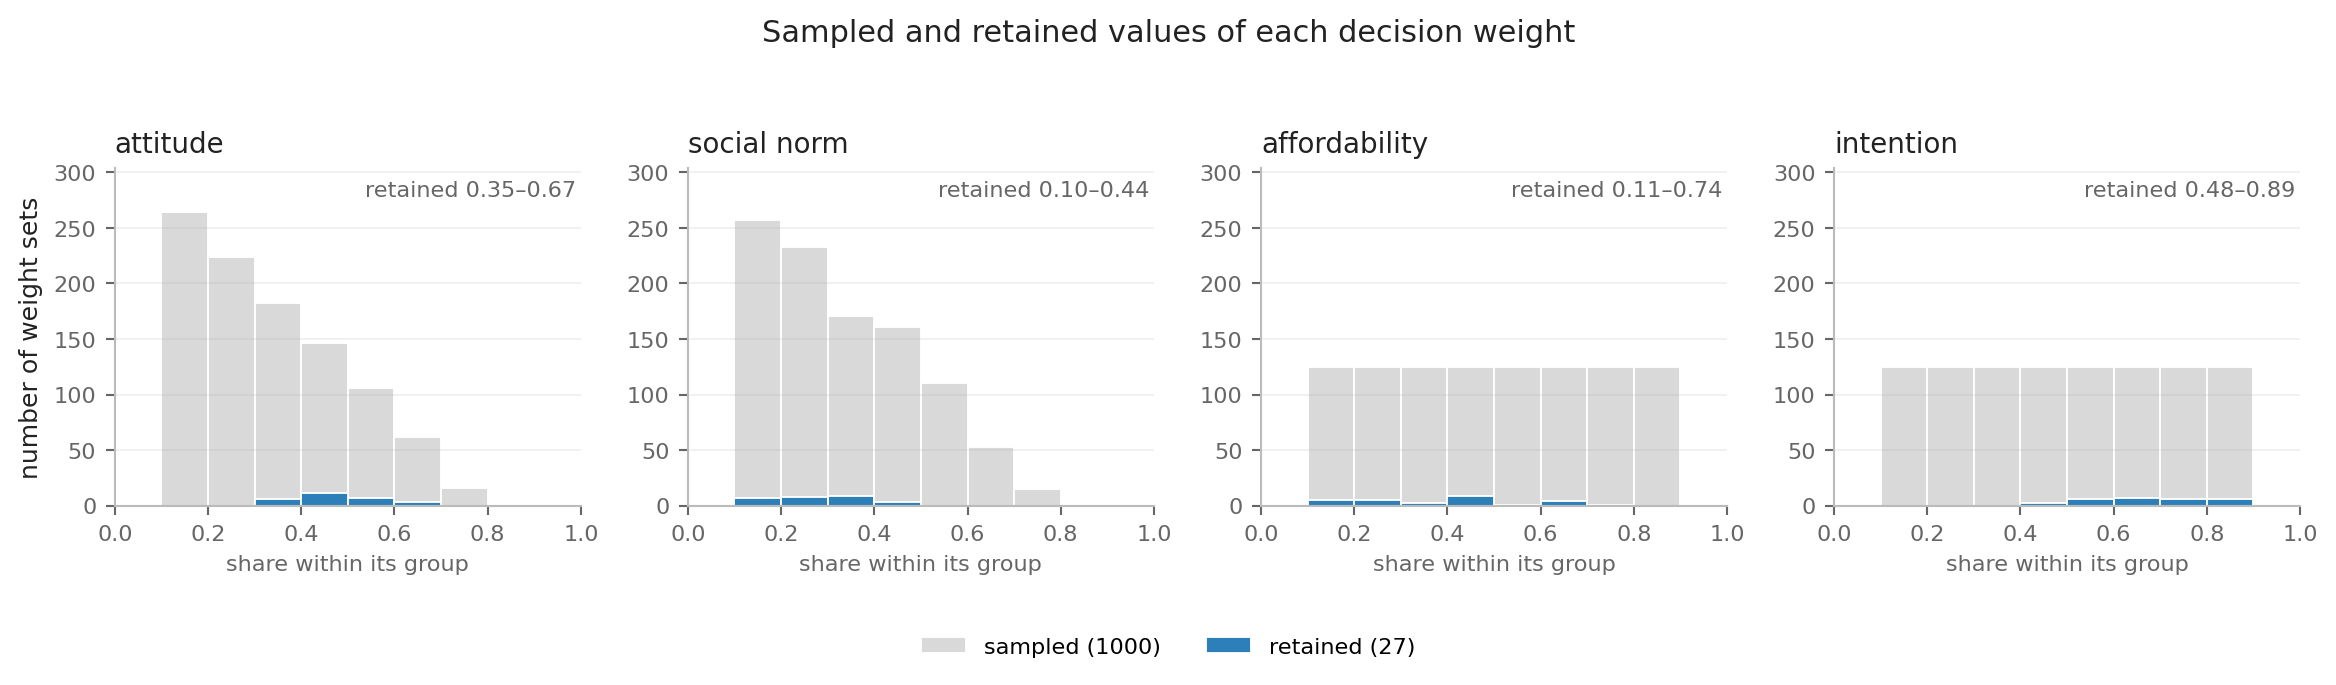
\includegraphics[width=\linewidth]{figures/fig_ensemble_weights.png}
%   \caption{Tested and retained weights of ensemble, showing that x and x require high weights}
%   \label{fig:ensemble_weights}
% \end{figure}

% \begin{figure}[htbp]\centering
%   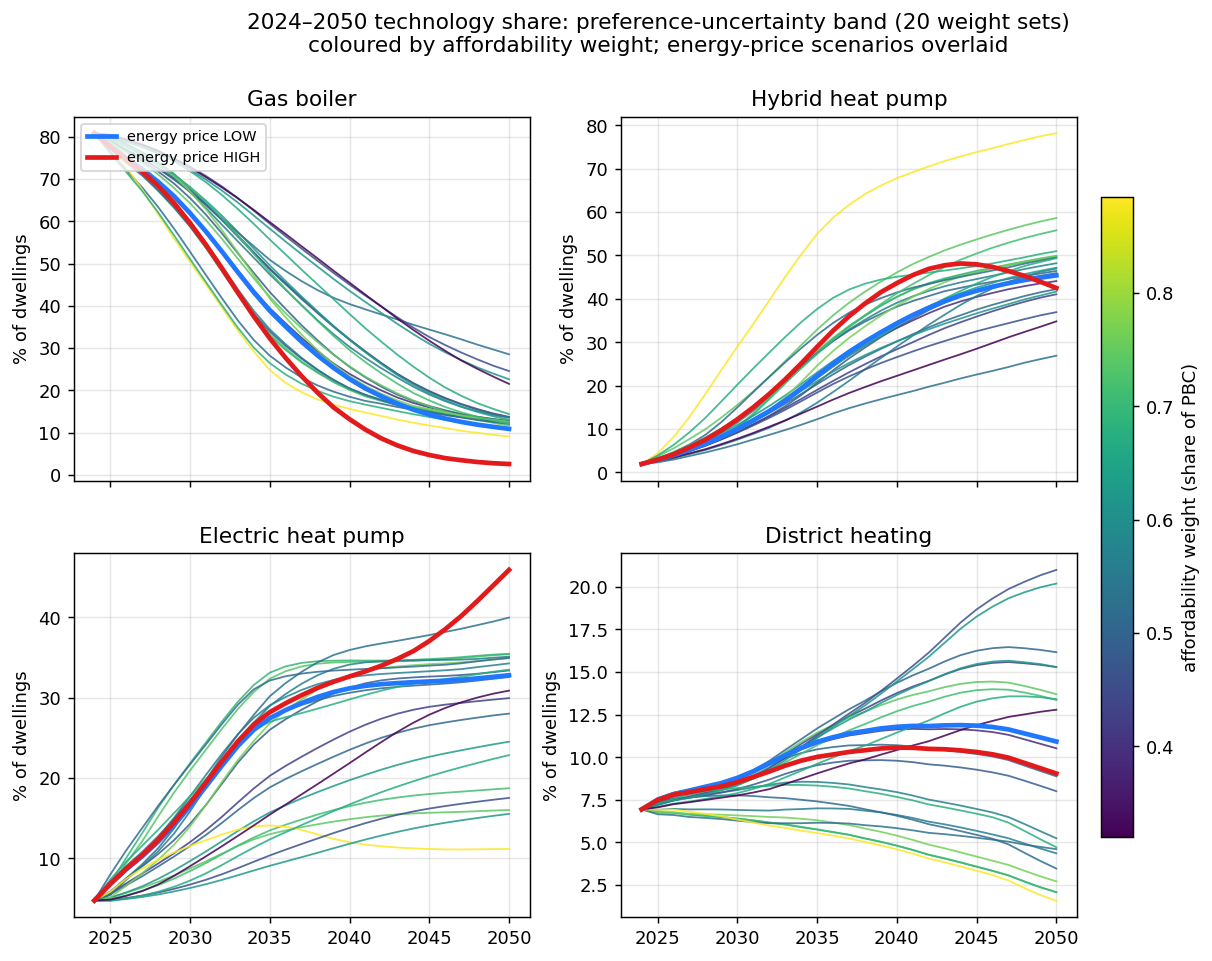
\includegraphics[width=\linewidth]{fig_band_affordability.png}
%   \caption{National technology-share pathways across the twenty-one member weight ensemble (baseline
%   scenario), coloured by the affordability weight, with the coupled energy-price scenarios overlaid.
%   Gas is displaced under every parameterisation; the split between the low-carbon options is not.}
%   \label{fig:band}
% \end{figure}

\begin{figure}[htbp]\centering
  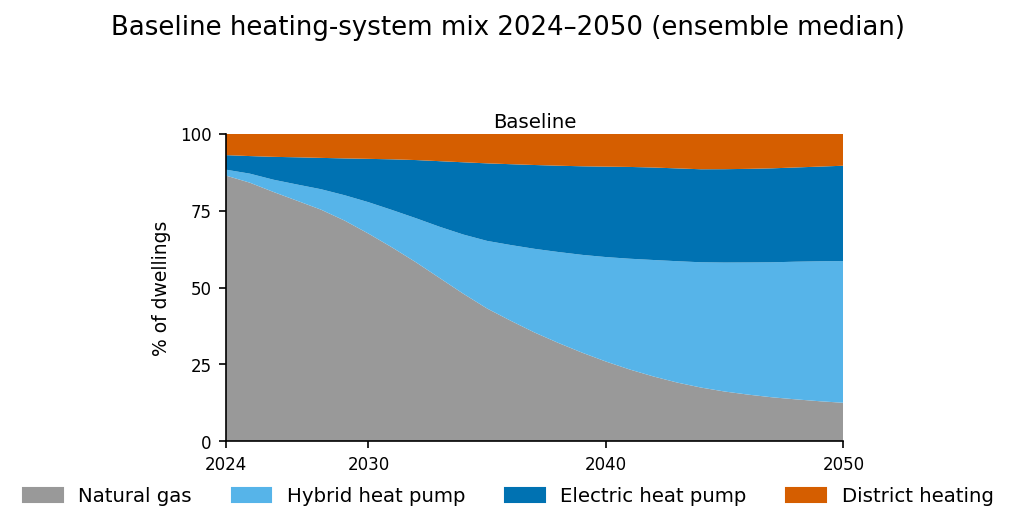
\includegraphics[width=0.62\linewidth]{figures/fig_scenario_mix_baseline.png}
  \caption{Baseline composition of the national heating stock, 2024--2050, as the median over the
  retained weight ensemble. The incumbent is displaced in every retained parameterisation; what
  replaces it is what the remaining sections are about. The same panel is drawn for every scenario
  in the design in Appendix~\ref{app:scenariogrid}.}
  \label{fig:mix_baseline}
\end{figure}

Figure~\ref{fig:mix_baseline} shows what this looks like as a pathway: gas retreats steadily from
2030 onward under every retained set, while the division of the remainder between hybrid heat pumps,
full electrification and district heating is what the scenarios and mechanisms move.

\paragraph{The techno-economic parameters are most influential on the long term}
Where attitude is key in matching behavior to historic trends, costs are key in determining
future pathways. The Morris analsys shows energy prices and learning rates to be by far the
key parameters, consistent over the three weight-sets (Figure~\ref{fig:morris}). Energy prices
largely determine the change between hybrid and electric, while also having influence on the 
remaining gas share. The adoption of district heating systems is not sensitive at all to the
tested parameters, showing that different policy measures, which will be tested in the scenarios,
are required. In the analysis it is most senstive to the randomness parameter describing which 
part is of decisions of home-owners are random, highlighting that there is little influence
of the decision-making algorithms. 

% Note, is this actually the case, and how does it relate to the social learning low and high scenario's which in the scenario analysis actually have far more deviation (but are not included that way in the sensitivity analysis I guess?)

% TODO: check this
% The ranking is stable across the preference space, so it is not an artifact of the weights
% chosen. A Latin-hypercube analysis confirms the directions and shows that the 2050
% electric heat-pump share is almost entirely explained by these economic factors ($R^2=0.91$),
% whereas the hybrid share is the least predictable ($R^2=0.60$), it is the swing technology that
% absorbs whatever the others do not take. This ranking sets the order of the mechanism sections
% that follow, and it is why the economic loop is examined first.

\begin{figure}[htbp]\centering
  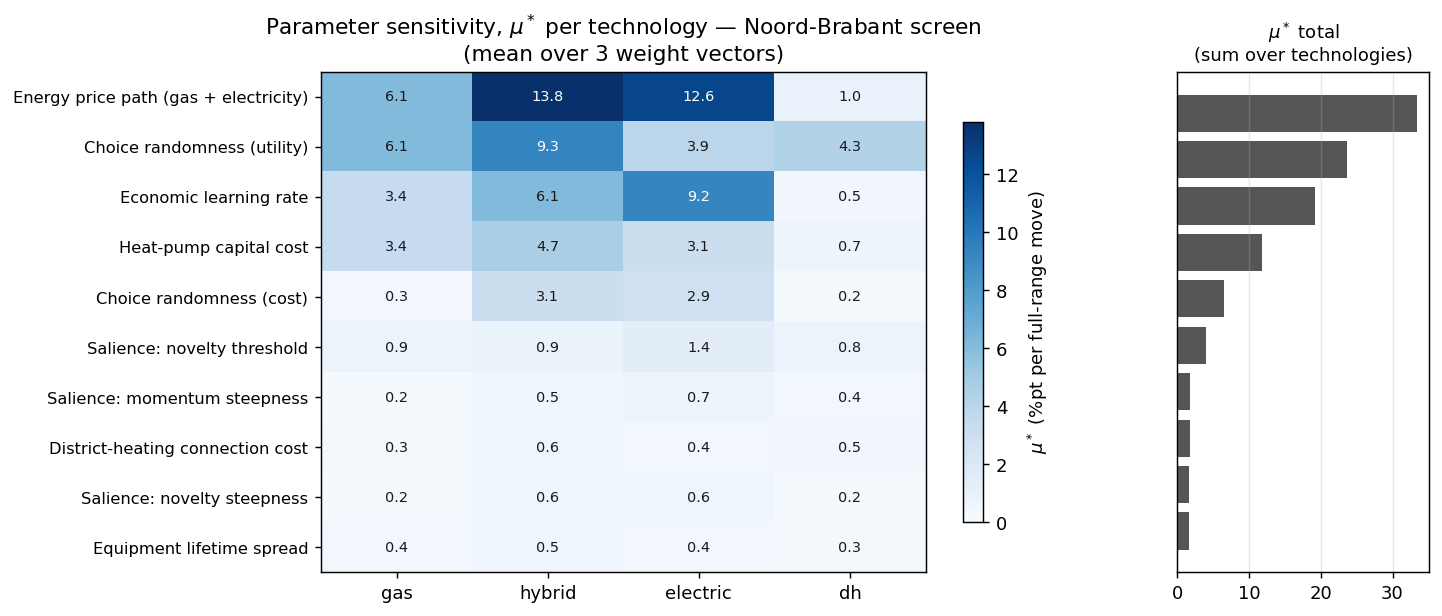
\includegraphics[width=0.9\linewidth]{figures/fig_structural_morris.png}
  \caption{Structural sensitivity of the 2050 heating mix (Noord-Brabant, averaged over three weight
  vectors spanning the retained ensemble). Energy prices and the learning rate
  dominate; the learning rate acts specifically on the hybrid-versus-electric split. 
  The screen is run on the calibration region because it requires several hundred model evaluations.}
  \label{fig:morris}
\end{figure}


\subsection{Feedback loops}
\label{sec:res-economic}

% Note to claude: check which feedback loops have most effect, insert the fig_Scenario_mix_grid for
% knock-outs on econ and social learning and the scenario's for high and low learning rates for both. Based on deviations here discuss the effects of both economic learning, and add how capex
% and energy price sensitivity relates to it.

Two kinds of experiment act on the learning loops. Figure~\ref{fig:mix_knockouts} severs each loop
in turn against an otherwise identical reference, which establishes whether the loop is causally
necessary. Figure~\ref{fig:mix_loops} varies the strength of each loop within its plausible range,
together with the coupled energy-price path through which the economic loop is driven, which
establishes how much of the outcome the loop can account for.

\begin{figure}[htbp]\centering
  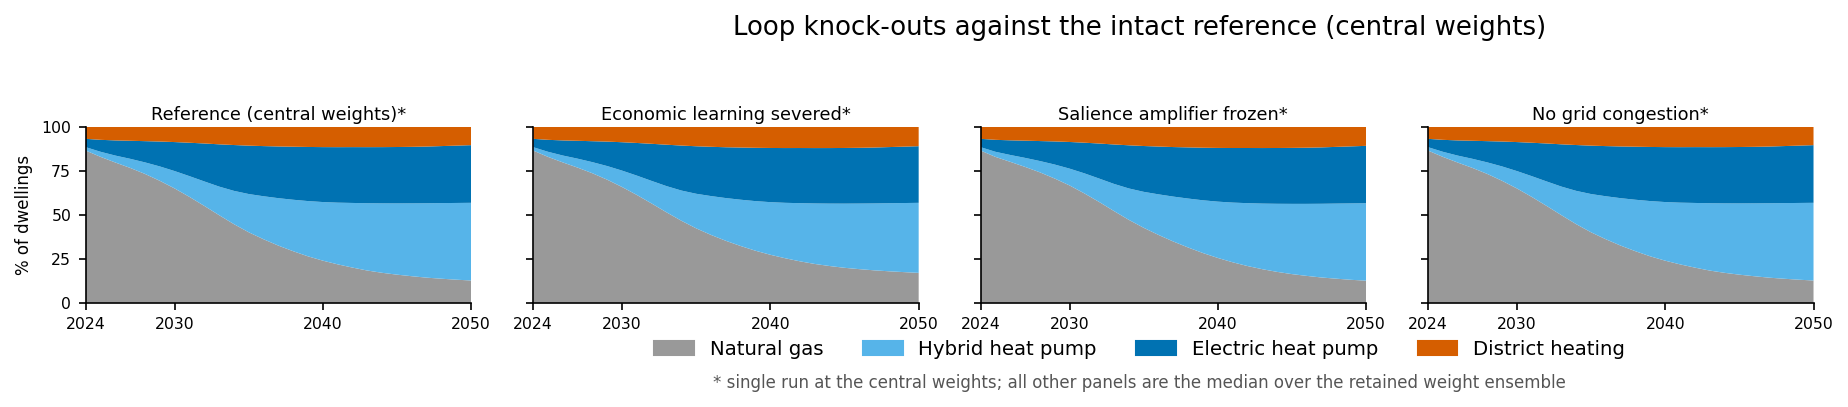
\includegraphics[width=\linewidth]{figures/fig_scenario_mix_knockouts.png}
  \caption{Loop knock-outs against their intact reference, all at the central weights. Each panel
  disables one element and leaves everything else identical, so the difference from the reference is
  that element's causal contribution. Severing economic learning holds 4.3 percentage points more of
  the stock on gas. Freezing the salience amplifier and removing the grid constraint change almost
  nothing; note that the salience freeze leaves each household's peer composition free to evolve and
  therefore bounds the amplifier rather than severing the diffusion loop.}
  \label{fig:mix_knockouts}
\end{figure}

Disabling the learning curve, holding capital costs at their initial values while leaving 
everything else identical, raises the 2050 gas share from 12.7\,\% to 17.0\,\% (Figure~\ref{fig:mix_knockouts}), with the
displaced demand falling back onto the hybrid heat pump (44.1 to 39.7\,\%) rather than onto full 
electrification, which is essentially unchanged (32.7 to 32.1\,\%). The reinforcing loop from 
installations to falling costs and back to installations is therefore a condition for the pace of
the transition, and specifically for the part of it carried by the cheaper technology. This mainly
influences landlords and SHA who have cost based decision-making algorithms.

Both heat-pump technologies show an extended acceleration phase in the late 2030s rather than a 
single sharp inflection. Locating the year of maximum acceleration identifies 2038 for both, but
the installation series carries year-on-year variation of the order of ten per cent,partly 
Monte-Carlo variability, partly the replacement cohorts created by finite equipment lifetimes. We 
therefore report an acceleration window of approximately 2036--2040 and treat the loop-state
trajectories, rather than a derivative, as the evidence that the feedback operates. Over the
period the learned capital cost falls 22.8\,\% for the hybrid and 32.3\,\% for the electric heat 
pump.

Energy prices are an independent axis of uncertainty. Because gas and electricity prices 
co-move, it is the spark spread rather than the price level that
governs the heat pump's running-cost advantage. Under the high-price path the 2050 electric 
heat-pump share reaches 45.9\,\% and gas falls to 2.6\,\%, while under the low-price path the mix
stays close to the static case (32.8 and 10.9\,\%). The high-price outcome lies outside the range
produced by any weight set at static prices (Figure~\ref{fig:mix_loops}): price uncertainty is not a 
subset of preference uncertainty but an independent axis that expands the envelope of attainable
futures.

\begin{figure}[htbp]\centering
  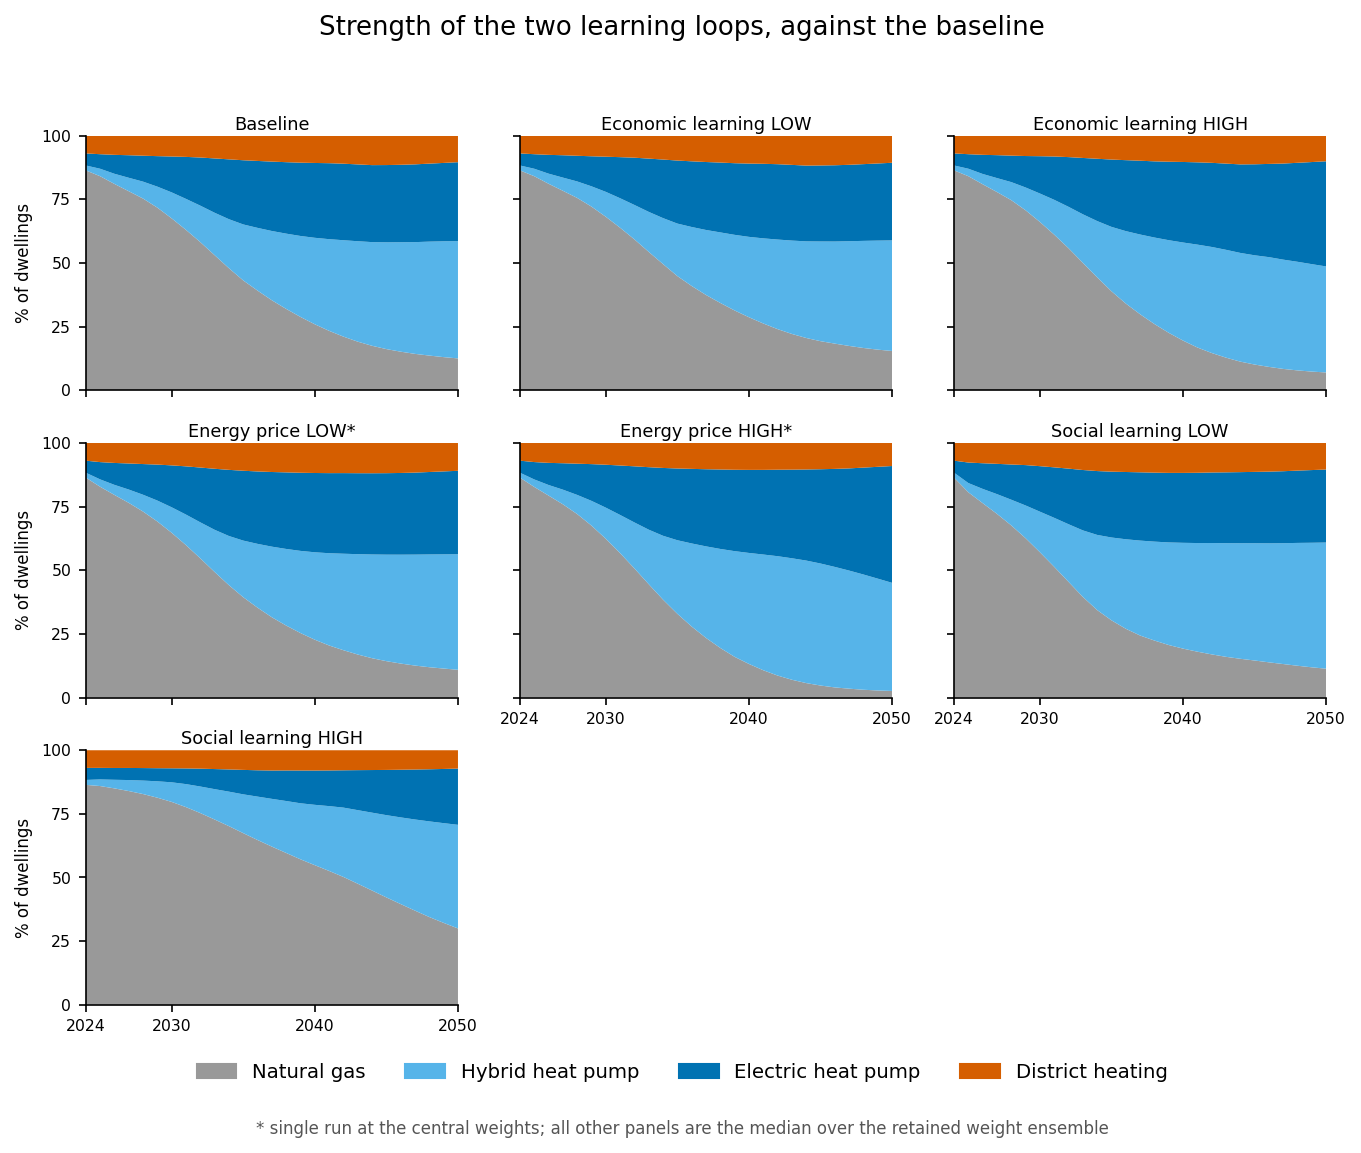
\includegraphics[width=\linewidth]{figures/fig_scenario_mix_loops.png}
  \caption{Strength of the two learning loops, against the baseline: the economic learning factor
  and the coupled energy-price path that drives the same loop, and the social learning factor. The
  shape of the transition is the same in all seven panels---gas is displaced and the heat pumps take
  the stock---but the composition is not: strong social learning leaves 31.3\,\% of dwellings on gas
  in 2050 against 2.6\,\% under the high price path.}
  \label{fig:mix_loops}
\end{figure}

\subsection{Social learning as a mechanism of incumbent lock-in}
\label{sec:res-social}

\paragraph{Amplified social influence entrenches the incumbent.}
The clearest result of the scenario set is counter-intuitive. Raising the social-learning factor does
not accelerate the transition: it \emph{reverses} it. With strong social learning the 2050 gas share
rises from 12.7\,\% to 30.6\,\% and the electric heat pump falls from 32.6 to 17.9\,\%, the largest
single-scenario deviation in either direction across the sixteen scenarios. Weakening social learning
has the opposite, if smaller, effect (gas 11.4\,\%).

The mechanism is straightforward once stated. Subjective norm is proportional to the share of a
household's peers already using a technology, and at the start of the simulation that share
overwhelmingly favours the incumbent: some four in five dwellings are heated by gas. Amplifying social
influence therefore amplifies, first and foremost, the advantage of gas. Social reinforcement is not
intrinsically progressive; it is conservative, and becomes an accelerant of low-carbon adoption only
after the peer base has been built by some other mechanism. In this model that other mechanism is
economic learning, which is why the two loops are asymmetric: cost decline can start a transition,
whereas social influence can only amplify whichever technology is already dominant.

\paragraph{Scope of the salience knock-out.}
% Note to claude: is this paragraph required, in general we need to see how the strucutural 
% sensitivity and the scenario analysis build on each other. In the scenario analysis the social
% learning feedback loop is absolute key.

Freezing the salience factor changes the 2050 mix by less than 0.3 percentage points. This is not
evidence that social influence is unimportant---the scenario result above shows the opposite---but a
limitation of that particular experiment: subjective norm is the product of peer-adoption share and
salience, and freezing salience leaves the peer-share term free to evolve, so the diffusion feedback
continues to operate. The knock-out therefore bounds the contribution of the salience \emph{amplifier}
rather than of social learning as such, and the social-learning scenarios provide the stronger
evidence.

\paragraph{Selectivity of social influence across adopter categories.}
Tracing adoption per adopter category shows the expected diffusion ordering---innovators lead,
laggards trail---but decomposing by technology reveals more (Figure~\ref{fig:segments}). The two heat
pumps are taken up by almost disjoint parts of the population. Innovators and early adopters end the
period on the electric heat pump with \emph{no} hybrid uptake at all (99.6 and 96.1\,\% electric,
0.0\,\% hybrid), whereas the late majority and laggards end predominantly on hybrids (57.6 and
59.0\,\%) with little or no electric uptake (21.3 and 0.0\,\%). The switchover is sharp and falls
between the early majority (82.5\,\% electric) and the late majority. District heating follows the
opposite gradient to the electric heat pump, rising monotonically from 0.4\,\% among innovators to
21.3\,\% among laggards.

Three consequences follow. First, an aggregate heat-pump curve conceals two opposing gradients and is
therefore uninformative about who adopts what. Second, the hybrid heat pump is not a laggard
technology in any pejorative sense but the \emph{majority} technology: it is the route by which the
late majority and laggards leave gas at all. District heating plays the same role for a smaller share,
consistent with collective supply serving households that will not invest individually. Third, the
only segment retaining significant gas in 2050 is the laggards (19.8\,\%); every other segment is
fully displaced.

This also explains a feature of the aggregate pathways that is otherwise puzzling. In most weight sets
the electric heat pump rises to a plateau and then grows little further; in the most cost-weighted sets
it peaks and then declines as early adopters replace electric units with hybrids at end-of-life. The
plateau is not a cost ceiling but \emph{segment saturation}: full electrification saturates the leading
adopter segments and the technically suitable dwellings, and then stops.

\begin{figure}[htbp]\centering
  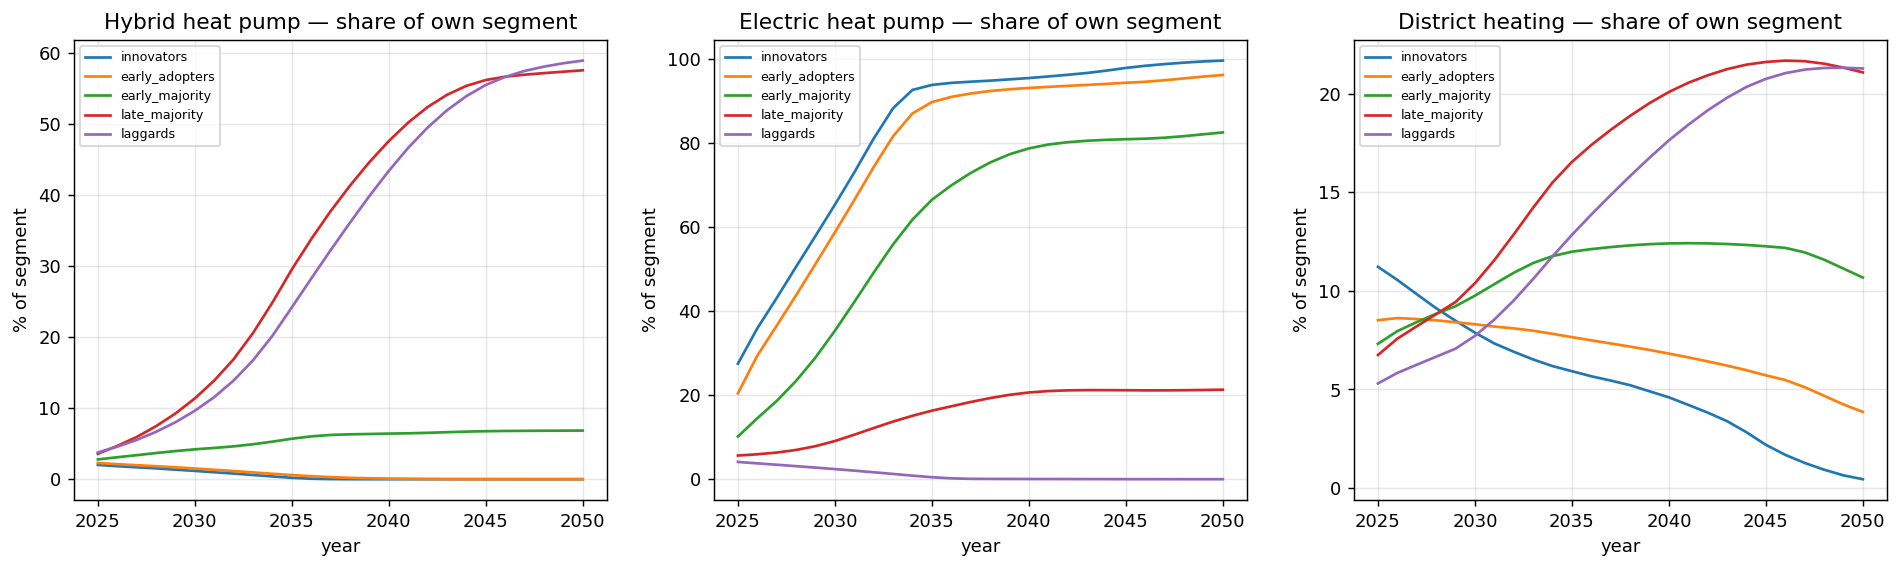
\includegraphics[width=\linewidth]{mech_segment_scurves.png}
  \caption{Adoption by adopter category, per technology, as a share of each segment's own stock. The
  hybrid and electric heat pumps follow opposite gradients---electric concentrating in the leading
  segments, hybrid in the trailing ones---while district heating follows the hybrid gradient. A
  combined heat-pump curve is nearly flat across segments because these gradients cancel.}
  \label{fig:segments}
\end{figure}

\paragraph{Ownership decides the route; dwelling characteristics only modulate it.}
Ownership separates the outcome far more sharply than any dwelling characteristic
(Figure~\ref{fig:segments_own}a). The 2050 electric heat-pump share is 31.5\,\% among
owner-occupied dwellings and 0.1\,\% in all three of the other ownership classes, which instead
take hybrids (60--84\,\%) and retain almost all residual gas (38.0\,\% privately rented and
27.6\,\% social housing, against 6.2\,\% owner-occupied). This is a direct consequence of the
decision rules rather than an emergent result: owner-occupiers decide through the full
behavioural function, in which attitude can outweigh an unfavourable cost comparison, whereas
landlords and housing associations minimise equivalent annual cost and therefore take the
cheapest compliant option, which is the hybrid. Owner associations are the one informative
exception. They minimise cost like the other landlords, but their stock is apartments and
high-rise, so the cheapest compliant option is more often a heat network: they end on 15.0\,\%
district heating, the highest of any ownership class, with no electrification at all.

\paragraph{Heat demand selects between individual and collective supply, not between capital and
operating cost.} Within the owner-occupied stock, where the behavioural function actually operates,
the expected cost logic---that high heat demand should justify the high-capital, low-operating-cost
electric heat pump---does not appear. The electric share is almost flat across demand tiers, at
29.3\,\% for low, 31.7\,\% for medium and 31.9\,\% for high demand, a spread of 2.6 percentage
points against the 31.4 points that ownership separates (Figure~\ref{fig:segments_own}c). What heat demand does move is the choice
between individual and collective supply: district heating falls from 22.8\,\% in low-demand
dwellings to 8.5\,\% in high-demand ones, and the hybrid rises correspondingly from 41.3 to
53.1\,\%. The same gradient survives conditioning on a single archetype, so it is not dwelling type
in disguise: within owner-occupied terraced houses alone, district heating falls from 17.5 to
9.5\,\% across the demand tiers while the electric share moves by one point.

Dwelling type acts through the same channel (Figure~\ref{fig:segments_own}d). Apartments and
high-rise end on 28.2 and 24.6\,\% district heating against 3.7\,\% for detached houses, and their
hybrid share is correspondingly lower, while the electric share varies only between 28.0 and
33.8\,\% across all six archetypes. Connection density, not the capital--operating cost trade-off,
is what dwelling characteristics contribute. Insulation label separates the outcome weakly and not
monotonically (Figure~\ref{fig:segments_own}e), and it cannot be read cleanly because the
segmentation does not cross label with ownership: the well-insulated stock is disproportionately
recent and rented, so the label gradient carries an ownership gradient inside it.

\paragraph{Adopter category orders the outcome inside the owner-occupied stock.} Among
owner-occupiers the adopter categories separate the 2050 outcome more sharply than ownership
separates the population as a whole (Figure~\ref{fig:segments_own}b). Innovators end almost entirely
on the electric heat pump (96.4\,\%) with no hybrid uptake at all; the gradient falls monotonically
to the laggards, who take no electric heat pumps, sit two-thirds on hybrids and hold the only
substantial residual gas in the owner-occupied stock (22.9\,\%). The switchover falls between the
early majority (46.0\,\% electric) and the late majority (6.1\,\%). District heating runs the
opposite way to the electric heat pump but far more weakly, from 3.6\,\% among innovators to
15.2\,\% among the late majority.

This gradient should be read as a description rather than as an explanation. The adopter category is
assigned by percentile of a propensity index built from the household's own sustainability attitude,
its network's mean attitude and the technical readiness of its dwelling, and attitude is also the
term in the decision function that carries adoption against an unfavourable cost comparison. A strong
gradient is therefore partly definitional. What it adds is the shape: the transition inside the
owner-occupied stock is not a uniform shift but a sequence, in which full electrification saturates
the leading segments and the hybrid is the route by which the trailing two thirds leave gas at all.
Ownership, by contrast, is exogenous stock data, which is why it is the structural divide and the
adopter gradient is the mechanism operating inside it.

The picture is therefore one determinant and one modifier. Ownership determines whether a dwelling
electrifies at all, because it determines which decision rule applies. Given that, the dwelling
determines whether the household is served individually or collectively, because it determines
whether a heat network is a credible option. Neither of these is a preference result: both follow
from structure the model imposes, which is why they hold across the weight ensemble.

\begin{figure}[htbp]\centering
  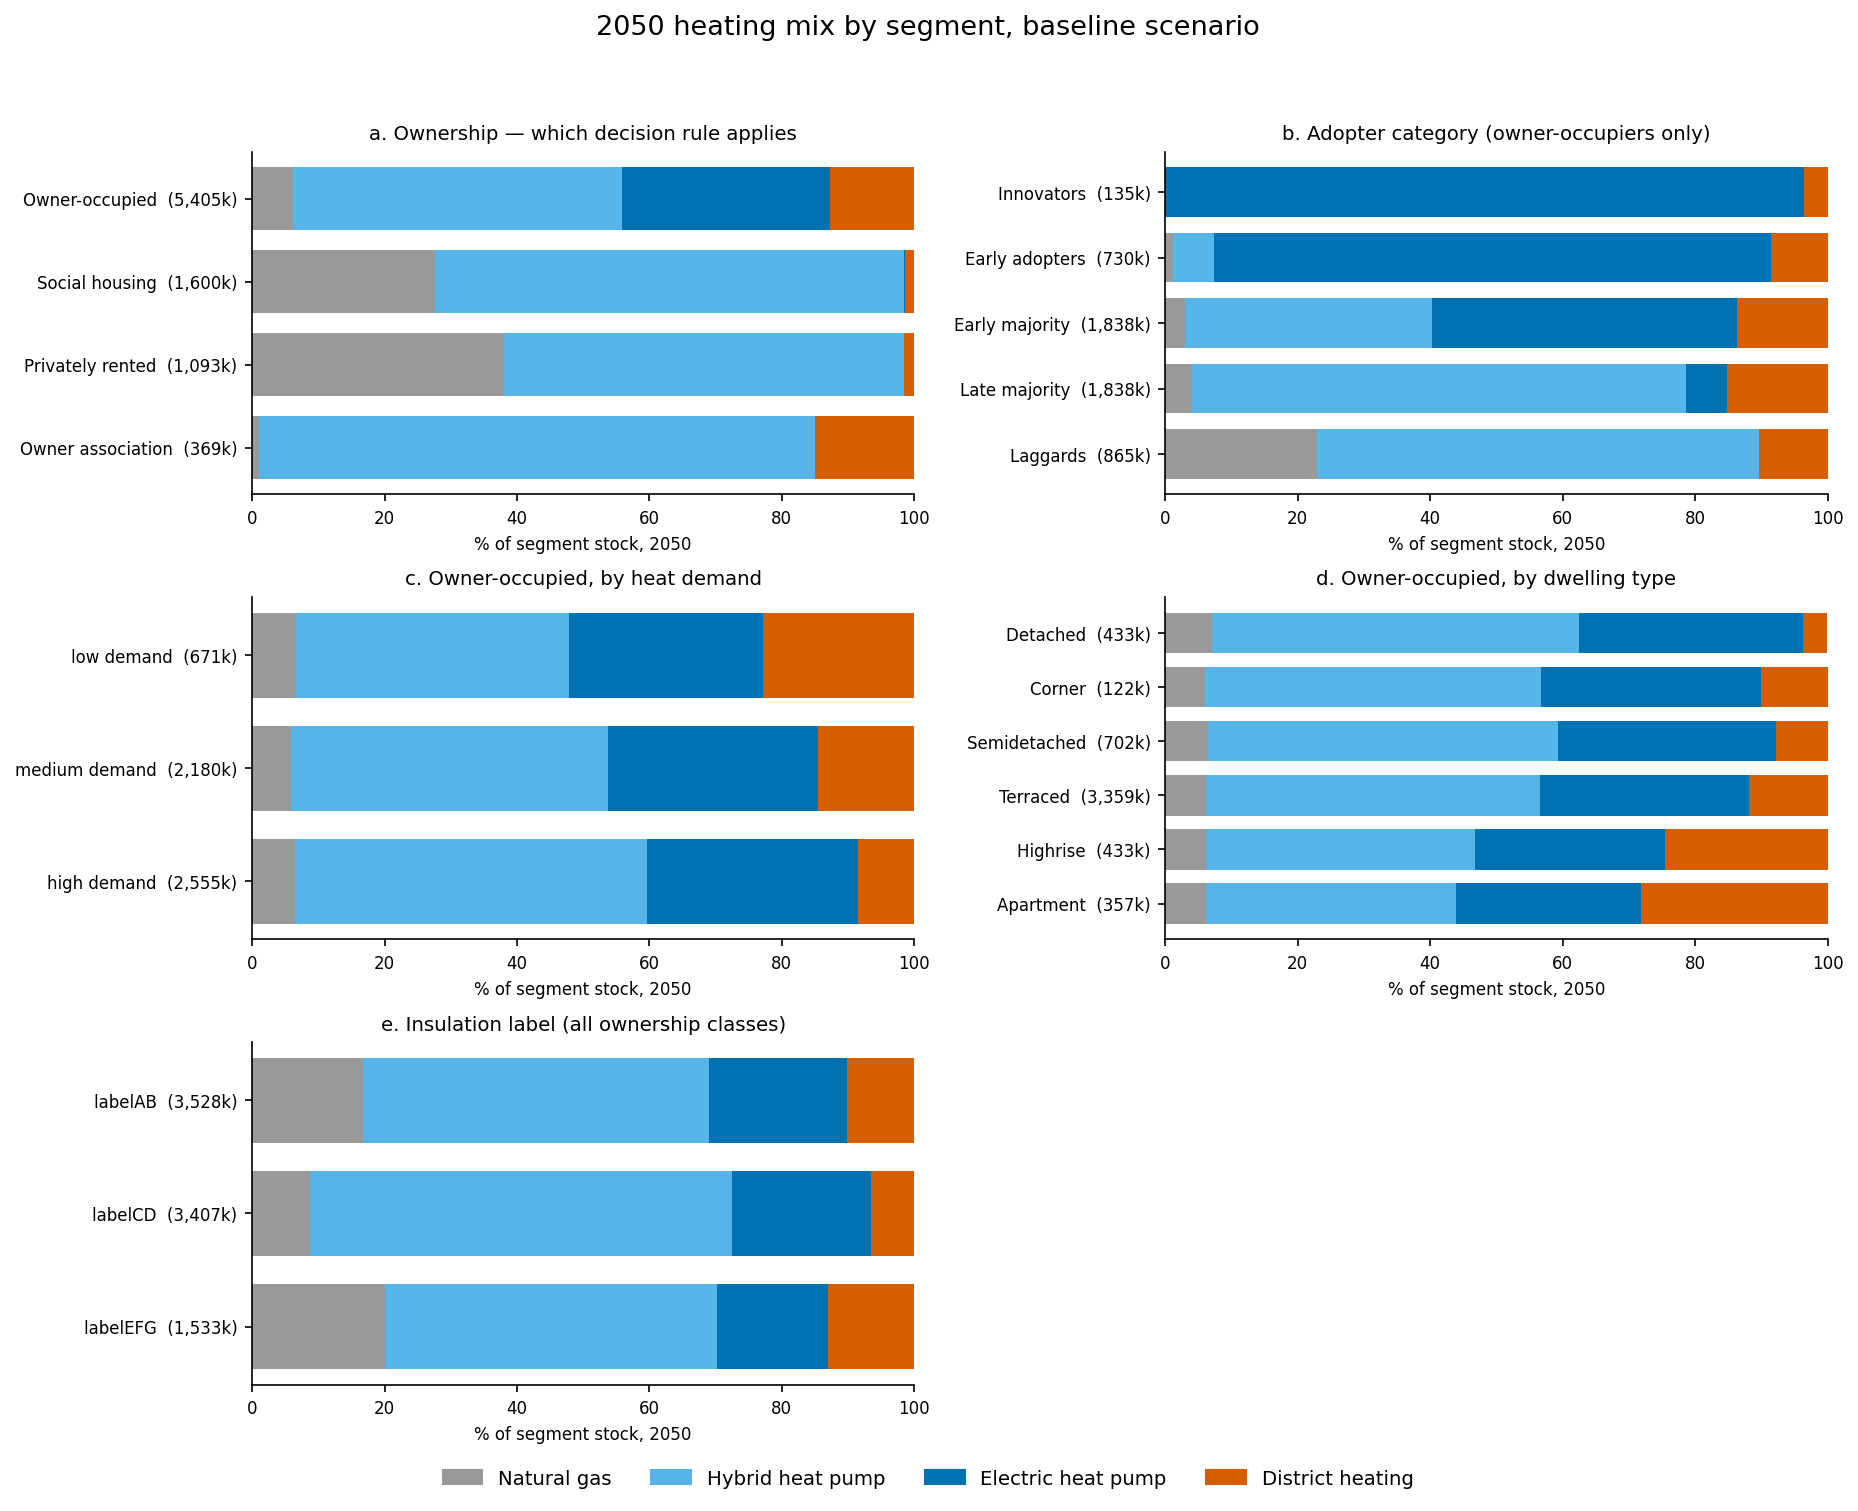
\includegraphics[width=\linewidth]{figures/fig_segments_ownership_dwelling.png}
  \caption{2050 heating mix by segment, baseline scenario, as a share of each segment's own stock.
  (a) Ownership, which sets the decision rule, separates electrification from non-electrification
  almost completely. (b) Adopter category, within the owner-occupied stock, separates it further
  still, though partly by construction (see text). (c, d) Heat demand and dwelling type shift the
  split between individual and collective supply while leaving the electric share nearly flat.
  (e) Insulation label pools all ownership classes and should be read with that confound in mind.}
  \label{fig:segments_own}
\end{figure}

\subsection{Rules, regulation and infrastructure}
\label{sec:res-rules}
% This is a key section, describing how much influence rules and regulations have on these feedback
% loops. Can we identify what has been triggered (how is DH triggered) in some cases (like HP ban)
% electric hp starts of well and is than blocked, what does it result in. Here insert the visuals
% of those scenario's relating to this section.

\begin{figure}[htbp]\centering
  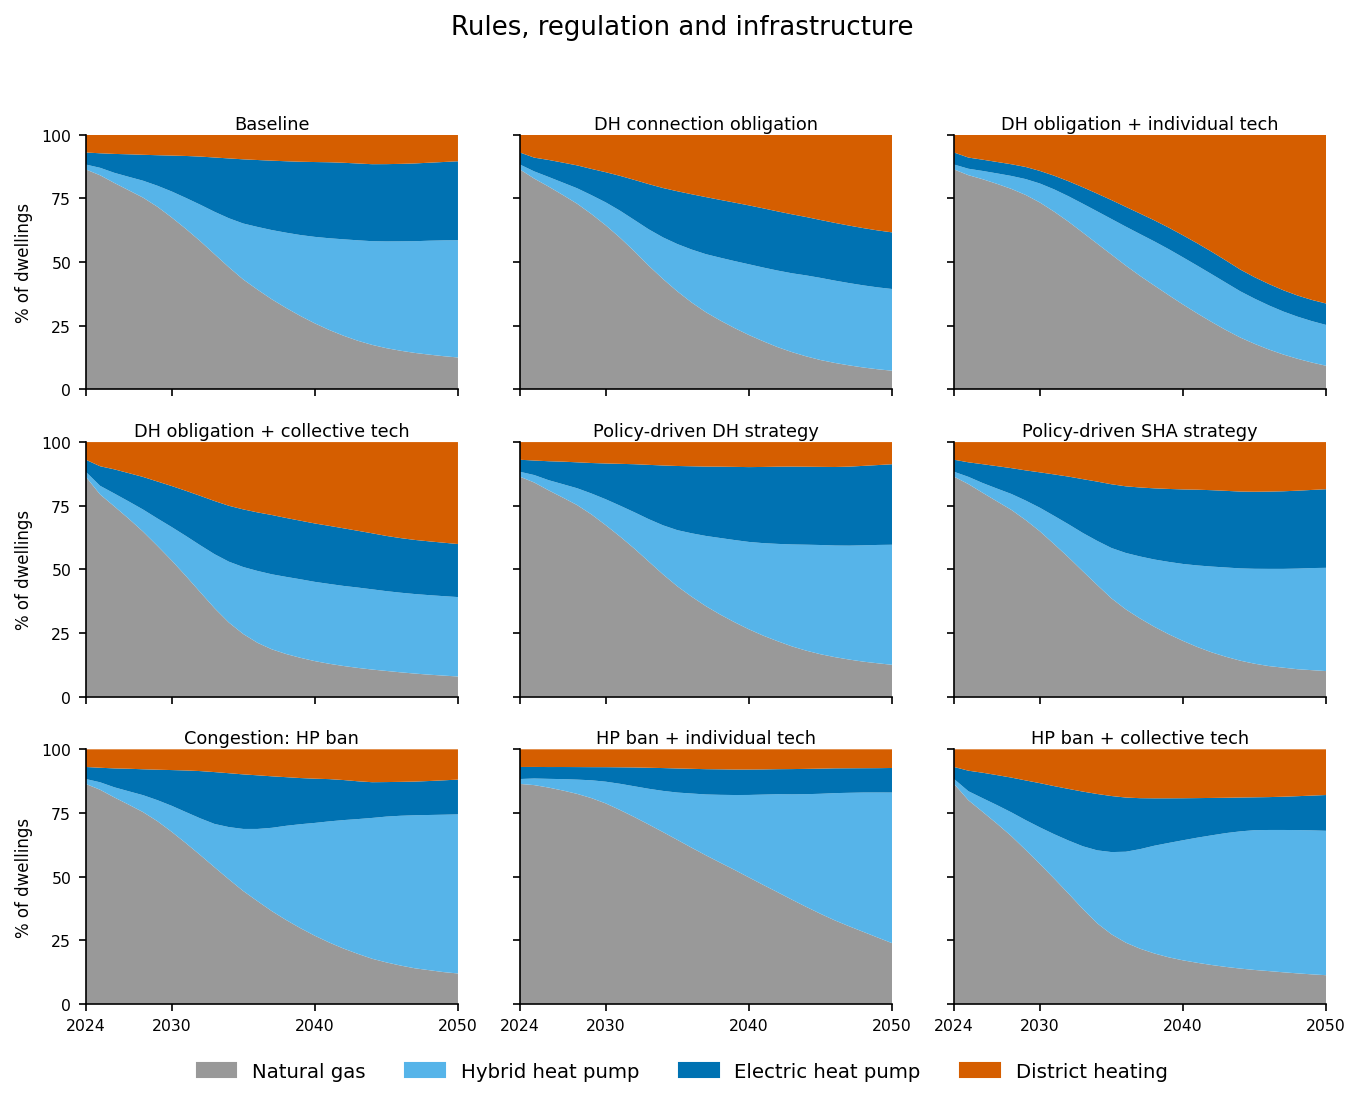
\includegraphics[width=\linewidth]{figures/fig_scenario_mix_policy.png}
  \caption{Rules, regulation and infrastructure, against the baseline. The connection obligation
  is the only lever that changes the composition of the 2050 stock substantially, and it does so by
  taking share from electrification rather than from gas. Directing network expansion without an
  obligation is indistinguishable from the baseline. The heat-pump ban reroutes adoption to hybrids
  instead of halting it.}
  \label{fig:mix_policy}
\end{figure}

Figure~\ref{fig:mix_policy} sets the four instruments against the baseline on common axes.

\paragraph{The district-heating connection obligation as the strongest single lever.}
Obliging dwellings in served neighbourhoods to connect raises the 2050 district-heating share from
8.9\,\% to 38.3\,\%, and to 63.1\,\% when combined with the individual-technology setting---the largest
effect of any intervention tested. It also lowers gas (to 7.4 and 9.9\,\%), but it does so by
displacing \emph{electrification} rather than gas alone: the electric heat-pump share falls by 10.4 and
24.8 percentage points respectively. The obligation is thus better read as a choice \emph{between}
decarbonisation routes than as an acceleration of decarbonisation as such.

\paragraph{Network expansion without an accompanying obligation.}
Directing district-heating companies to follow the municipal transition plans, without an accompanying
connection obligation, moves the 2050 mix by less than one percentage point on every technology. The
binding constraint is not where networks are built but whether households connect to them. This is the
threshold logic of the mechanism: a network requires a critical connection density to be viable, and a
plan that builds capacity without securing demand does not cross it.

\paragraph{Grid congestion as a redirecting rather than a blocking constraint.}
A heat-pump ban in congested neighbourhoods lowers the electric heat-pump share from 32.6 to 13.8\,\%
while the hybrid share rises from 47.2 to 63.5\,\%, with gas almost unchanged (12.1\,\%). The
constraint therefore reroutes the transition rather than halting it: households prevented from
installing an electric heat pump take a hybrid, not a gas boiler. Congestion is measured in every
scenario but constrains choice only where policy makes it binding, reflecting that a distribution
operator cannot in practice prevent a household from installing within its existing connection
capacity; the scenario is illustrative of the mechanism rather than a forecast of grid constraints.

\subsection{Coordination between collective actors}
\label{sec:res-coordination}

\begin{figure}[htbp]\centering
  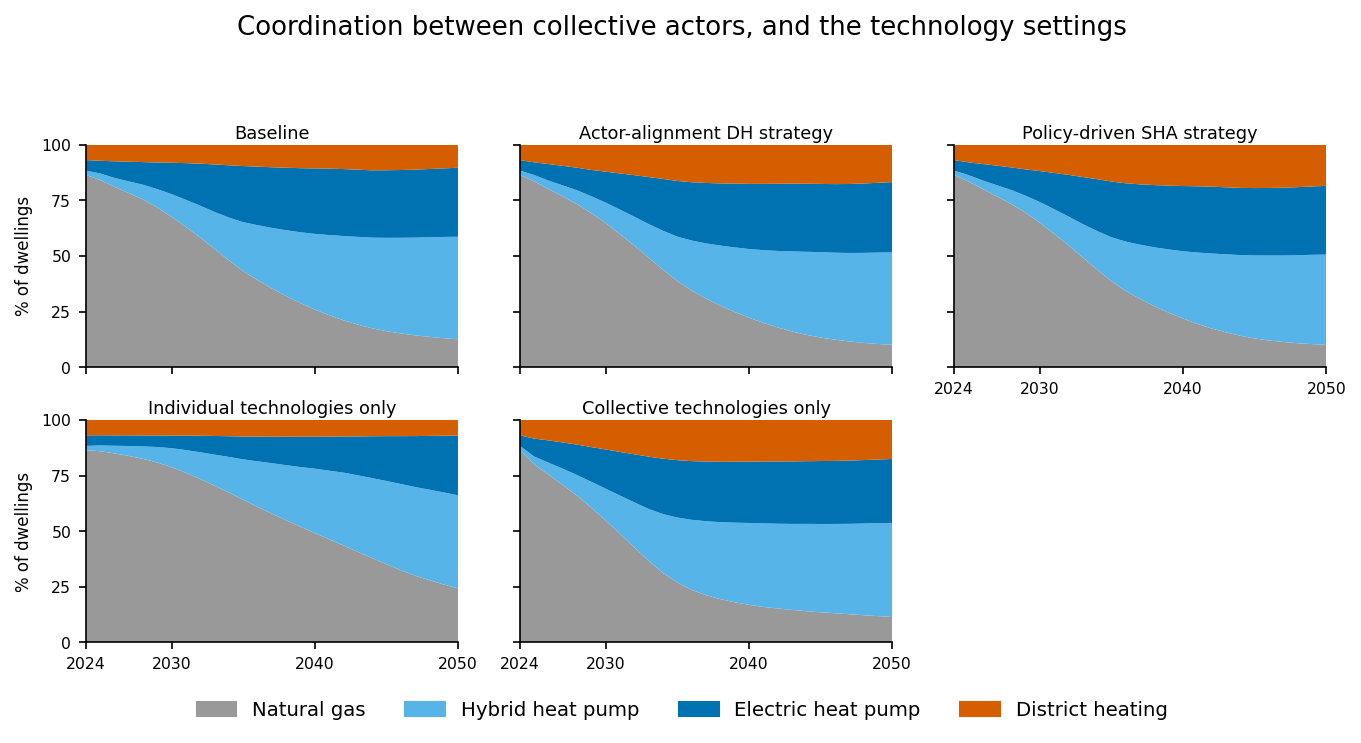
\includegraphics[width=\linewidth]{figures/fig_scenario_mix_coordination.png}
  \caption{Collective-actor coordination and the technology settings, against the baseline. Most of
  the coordination effect comes from the housing associations rather than from the network
  companies, and the individual-technology setting raises the residual gas share rather than
  lowering it.}
  \label{fig:mix_coordination}
\end{figure}

Aligning the collective actors---district-heating companies and housing associations both following
municipal plans (Figure~\ref{fig:mix_coordination})---lowers the 2050 gas share from 12.7 to 10.1\,\% and raises district heating from 8.9
to 16.1\,\%, with full electrification unchanged. Social-housing strategy alone achieves nearly the
same (10.2 and 17.3\,\%), indicating that most of the coordination benefit comes from the housing
associations rather than from the network companies. This is consistent with the tenure result above:
associations control a large, spatially concentrated stock that they convert as a block, which is
precisely the demand density a heat network requires.

The combined technology scenarios are more revealing than either alone. The collective-technology
setting lowers gas modestly (11.5\,\%) and raises district heating (17.1\,\%), whereas the
individual-technology setting---strong social \emph{and} economic learning together---\emph{raises} the
2050 gas share to 24.3\,\%. The social lock-in identified above dominates the economic acceleration
when both are strengthened simultaneously. Coordination between actors is therefore not merely additive
with the learning mechanisms: it interacts with them, and the sign of the interaction depends on
whether the incumbent still holds the social advantage.

\subsection{Synthesis: the asymmetry of the mechanisms}
\label{sec:res-synthesis}

Across all mechanisms the model gives a consistent account of what is robust and what is not. Gas
heating is displaced under every plausible parameterisation; the uncertainty lies in the route, and the
spread between routes is several times larger than the spread in the residual gas share.

The mechanisms are asymmetric in a way that matters for policy. Economic learning is the only mechanism
that can \emph{start} a transition: it is causally necessary, its parameters dominate the structural
sensitivity, and the price and capital-cost levers that act on it move the outcome beyond the entire
preference band. Social learning cannot start a transition and, when strengthened while the incumbent
still holds the peer majority, actively entrenches it. Infrastructure policy---specifically a
connection obligation---is the strongest single lever available, but it selects a route rather than
accelerating decarbonisation in general.

Who is reached differs by route. Full electrification is an owner-occupier and early-adopter
phenomenon that saturates its available segments; hybrids and district heating are the routes by which
the majority, and particularly rented and social housing, leave gas at all. Policies that lower
heat-pump costs or widen the spark spread accelerate the transition; policies that oblige connection
redirect it; and policies aimed at tenure---at the landlords and associations who minimise cost rather
than weigh attitude---determine whether the majority of the stock electrifies or hybridises.

%% ===========================================================================
\section{Discussion}
%% ===========================================================================

% NOTE: this section was in bullet-point/outline form in the source draft.
% Retained as bullets; convert to prose when ready.
\begin{itemize}
  \item In this paper we show how bottom-up modelling can be done to explore large,
    real-world systems and transition pathways.
  \item Including individual agent decision-making in heterogeneous populations.
  \item This leads to non-linear adoption behaviour.
  \item Giving the potential to explore the solution space.
  \item And the potential to add all kinds of tipping dynamics such as economies of
    scale in the case of district heating, and coevolution leading to
    infrastructure bottlenecks such as grid congestion.
  \item However, these models should be used with caution. Decision-making
    strategies of all actors involved are much more elaborate and context specific.
    People use different decision-making strategies \citep{michelsenMotivationalFactorsInfluencing2013}
    with extreme heterogeneity \citep{melesHeterogeneityPreferencesRenewable2022}. This will evolve throughout
    different contexts and could evolve over time. Especially difficult and
    impactful decisions such as a dwelling heating method would usually be a
    multi-stage decision process in which the decision-makers' thought process
    evolves over time and through social discourse and investigation.
  \item The inherent uncertainty of such decision-making processes has resulted in
    omitting them in most energy transition pathways. We argue it is better to
    include them and explore the potential impact of these drivers throughout a vast
    range of scenarios.
\end{itemize}

% ===========================================================================
% DRAFT Discussion + Conclusion. Replaces \section{Discussion} and
% \section{Conclusion}. Written from the national ensemble results.
% Marked [CHECK] where a claim should be verified against the literature
% before submission.
% ===========================================================================

\section{Discussion}
\label{sec:discussion}

\subsection{Social reinforcement favours the incumbent}

The result with the widest implications is that strengthening social learning slows the transition
rather than accelerating it, raising the 2050 gas share from 12.7 to 30.6\,\%. This runs against the
common framing of social influence as a lever for accelerating low-carbon adoption, in which peer
effects and social norms are treated as mechanisms to be amplified
\citep{wiedermannNetworkbasedMicrofoundationGranovetters2020,lentonOperationalisingPositiveTipping2022/ed}.

The apparent contradiction dissolves once the direction of the mechanism is made explicit. Social
influence is a function of what peers currently do, and at the start of a transition what peers
currently do is overwhelmingly the incumbent practice. Amplifying conformity therefore amplifies the
incumbent's advantage first. The literature on social tipping generally analyses the regime
\emph{after} a critical mass has formed, where reinforcement does accelerate adoption; our results
concern the regime before it, where the same mechanism operates in reverse. Social influence is better
characterised as conservative than as progressive: it entrenches whatever is already majority
practice, and becomes an accelerant only once the peer base has been built by some other mechanism.

This has a practical consequence. Interventions designed to strengthen social signals---visibility
campaigns, neighbourhood demonstration effects, peer comparison---should be expected to help only where
low-carbon adoption already has local majority status, and to be counterproductive where it does not.
The implication is not that such interventions are useless but that their timing and spatial targeting
matter more than their strength. [CHECK: position against the social-tipping literature, which
typically assumes the post-critical-mass regime; \citet{milkoreitSocialTippingPoints2023} may be the
right anchor.]

\subsection{Two loops, and only one of them can start a transition}

The two reinforcing loops are not interchangeable. Economic learning is causally necessary: disabling
it leaves roughly a third more dwellings on gas, its parameters dominate the structural screen at every
point of the preference space we tested, and the levers acting on it---capital cost, learning rate and
the gas-to-electricity price ratio---move the 2050 outcome beyond the entire band produced by
preference uncertainty. Social learning, by contrast, can amplify but not initiate.

This asymmetry suggests a sequencing argument. Cost-side intervention is a precondition; social-side
intervention is a multiplier that only pays once the cost-side work has produced a local majority. A
policy programme that leads with the social instruments risks reinforcing the incumbent, whereas one
that leads with cost and follows with social instruments compounds. The tipping-point framing that
motivates this paper is therefore incomplete if it treats reinforcing loops as equivalent: the question
is not only whether a loop exists but whether it can act on a minority technology.

\subsection{The route is uncertain even where the destination is not}

Across the ensemble, gas is displaced in every parameterisation, but the low-carbon mix ranges from
hybrid-dominated to electric-dominated to district-heating-dominated. Because these routes differ in
their infrastructure requirements, their residual gas consumption and the households they reach, this
is not a second-order uncertainty. A hybrid-dominated pathway retains a gas connection and a
gas-consuming appliance in a majority of dwellings; a district-heating-dominated pathway requires
network investment concentrated in dense areas; a fully electrified pathway loads the distribution
grid. Planning that assumes a single route risks stranding the infrastructure built for it.
[CHECK: quantify residual gas demand per route---the model records it and it would strengthen this
paragraph considerably.]

The practical reading is that the near-term policy question is less "how fast" than "toward what". The
connection obligation illustrates this sharply: it is the strongest lever we tested, but it works by
displacing electrification rather than by displacing gas, moving the system between low-carbon routes
rather than further from the incumbent.

\subsection{Tenure is the binding structural divide}

Full electrification is concentrated almost entirely in owner-occupied dwellings (50.8\,\% versus
0.7--1.2\,\% elsewhere), and the residual gas in 2050 is concentrated almost entirely in rented and
social housing (29.9 and 38.3\,\% versus 3.2\,\%). This follows from the decision rules---owner-occupiers
weigh attitude alongside cost, whereas landlords and associations minimise cost---and it reproduces the
split-incentive problem familiar from the energy-efficiency literature
\citep{jakobChapterOverviewSector2020}. [CHECK: connect explicitly to the split-incentive/landlord-tenant
literature.]

The policy implication is that instruments aimed at households are aimed at the segment that is already
transitioning. The segments that retain gas respond to cost, not to attitude or social signal, so the
instruments that reach them are those that change the landlord's or association's cost calculus:
standards, subsidy conditionality, or obligation. This also qualifies the adopter-category result: the
Rogers ordering that the model reproduces is, to a substantial degree, a tenure ordering in disguise.

\subsection{Limitations}

Several limitations bear on how far these results should be read.

\emph{The calibration window is short and atypical.} Three years of observed adoption cannot identify
the decision weights uniquely, which is why we report an ensemble rather than a fitted parameterisation;
the window also coincides with unusually strong subsidies and a gas-price shock, so weights fitted to it
may absorb transient drivers.

\emph{Structural uncertainty is not quantified.} We vary parameters, not model form. Whether the theory
of planned behavior is the right account of the adoption decision, or the S-curve the right description
of social visibility, is not tested here, and the sensitivity results are conditional on those choices.

\emph{Matching the recent past does not validate the projections.} The calibration filters out
behaviourally implausible parameterisations; it does not establish that the 2050 pathways are correct.
They are interpreted for the mechanisms they reveal, not as forecasts.

\emph{Some mechanisms are represented schematically.} Grid congestion constrains choice only where
policy makes it binding; district-heating expansion uses a single density threshold; and roughly a
quarter of neighbourhoods lack observed heating data and are initialised as gas-heated. Heat demand
responds to insulation but not to occupant behaviour, and the salience knock-out bounds only the
amplifier term rather than the full social feedback.

\section{Conclusion}
\label{sec:conclusion}

We set out to identify where path dependency and tipping dynamics arise in the Dutch residential heat
transition, and which mechanisms govern them. Using an agent-based model calibrated by history matching
against observed 2022--2024 adoption and run across a twenty-one member weight ensemble, three
conclusions hold across the plausible parameter space.

First, \textbf{the displacement of gas heating is robust but the route is not}. In every
parameterisation the gas boiler falls to roughly a tenth of the stock by 2050, yet the low-carbon mix
ranges from hybrid-dominated to electric-dominated to district-heating-dominated. The uncertainty that
matters for planning is not whether the incumbent is displaced but what replaces it, because the routes
differ in infrastructure, residual gas use and the households they reach.

Second, \textbf{the two reinforcing loops are asymmetric, and only economic learning can initiate a
transition}. Disabling the learning curve leaves substantially more dwellings on gas, and the
cost-side parameters dominate the structural sensitivity at every point of the preference space tested.
Strengthening social learning, by contrast, \emph{raises} the 2050 gas share by eighteen percentage
points, because social influence amplifies whatever is currently majority practice and the incumbent
begins with that majority. Social reinforcement is a multiplier on an existing direction, not a source
of one.

Third, \textbf{the transition is segmented by technology and by tenure rather than merely paced}. Full
electrification is an owner-occupier phenomenon that saturates the leading adopter segments and then
stops; hybrids and district heating are the routes by which the late majority, and particularly rented
and social housing, leave gas at all. The residual gas in 2050 sits almost entirely in the rented stock.

For policy, these results suggest that sequencing matters as much as instrument choice. Cost-side
measures are a precondition rather than one option among several; social instruments repay investment
only where low-carbon adoption already holds a local majority; and the strongest single lever we
tested---a district-heating connection obligation---selects a route rather than accelerating
decarbonisation in general. Because the segments retaining gas respond to cost rather than to attitude
or social signal, instruments directed at landlords and housing associations are likely to determine
whether the majority of the stock electrifies, hybridises, or remains on gas.

Further work should extend the analysis in three directions: quantifying structural as well as
parametric uncertainty by testing alternative decision-model forms; representing the grid constraint
physically rather than as a policy-activated rule; and resolving the spatial dimension of the threshold
mechanisms, since both district-heating viability and congestion are defined per neighbourhood and are here reported only in aggregate.

%% ===========================================================================
\section{Conclusion}
%% ===========================================================================

% TODO: conclusion to be written.

%% ===========================================================================
%% Bibliography
%% ---------------------------------------------------------------------------
%% Style: elsarticle-harv = author-year (matches the (Author, Year) style of the
%% original manuscript). For a numbered journal, swap to elsarticle-num and
%% change the class option `authoryear' to `number' at the top of this file.
%% ---------------------------------------------------------------------------
\bibliographystyle{elsarticle-harv}
\bibliography{references}

%% ===========================================================================
\clearpage
\appendix
%% ===========================================================================

\section{Model documentation}
\label{app:model}
 
This appendix documents the model following the ODD (Overview, Design concepts,
Details) protocol \citep{grimmODDProtocolReview2010}. Cost, learning and scenario
details are given in Appendices~\ref{app:cost}--\ref{app:grid}; here we summarize the
structure and refer back to the main text for the decision equations.
 
\subsection{ODD protocol}
\label{app:odd}
 
This section documents the model following the ODD (Overview, Design concepts,
Details) protocol \citep{grimmODDProtocolReview2010}. To avoid duplication, decision
equations are referenced from Section~\ref{sec:model} and the cost, learning and
scenario submodels from Appendices~\ref{app:cost}--\ref{app:grid}.
 
\subsubsection{Overview}
 
\paragraph{Purpose and patterns}
The purpose of the model is to explore how path dependency, lock-ins and tipping
points emerge in the Dutch residential heat transition, and how policy measures and
actor strategies shape the resulting 2024--2050 heating-technology pathways. It is a
tool for understanding mechanisms and mapping plausible pathways under uncertainty,
not for point prediction. The model is expected to reproduce a set of stylized
patterns that give it structural credibility: (i) S-curve diffusion of individual
low-carbon heating technologies driven by cost decline and social influence;
(ii) threshold (increasing-returns) behavior in collective district-heating roll-out;
(iii) heterogeneity in adoption timing across household types and dwelling
characteristics; and (iv) the direction and magnitude of the observed 2022--2024
change in the provincial heating mix, which is used as a plausibility filter during
calibration (Section~\ref{sec:calibration}).
 
\paragraph{Entities, state variables and scales}
The model contains six entity types---dwellings, homeowners, social housing
associations, landlords, a district heating company and an electricity grid
operator---plus neighborhoods as the spatial unit at which collective (grid and
district-heating) decisions are made. Table~\ref{tab:odd-state} lists the principal
state variables per entity. Global state comprises, per heating technology, the
learning-updated investment cost, cumulative installed units, energy price and
salience factor. The model advances in annual time steps over 2024--2050 (and over
2022--2024 for calibration). The spatial extent is a single province (the calibration
and analysis scope, e.g.\ Noord-Brabant) or the full Netherlands ($\sim$8~million
dwellings); dwellings are geolocated to neighborhoods but not to coordinates.
 
\begin{table}[htbp]
  \centering
  \caption{Principal state variables by entity. Variables marked $\ast$ change during
  a run; others are set at initialization.}
  \label{tab:odd-state}
  \footnotesize
  \begin{tabular}{L{3.0cm} L{9.4cm}}
    \toprule
    \textbf{Entity} & \textbf{State variables}\\
    \midrule
    Dwelling & construction year, type, floor area, ownership, energy label$\ast$,
      in-house heat-distribution system$\ast$, current heating method$\ast$, system
      age$\ast$, drawn end-of-life age, heat demand.\\
    \addlinespace
    Homeowner & sustainability attitude, peer network, per-method attitude, subjective
      norm$\ast$ and perceived behavioral control$\ast$, resulting intention$\ast$ and
      utility$\ast$.\\
    \addlinespace
    Social housing assoc.\ / landlord & set of owned dwellings, adoption strategy
      (cost- or policy-based, for associations).\\
    \addlinespace
    District heating company & expansion strategy, per-neighborhood grid state$\ast$,
      construction lead time.\\
    \addlinespace
    Grid operator & per-neighborhood peak demand$\ast$ and congestion state$\ast$,
      reinforcement rate.\\
    \addlinespace
    Neighborhood & dwelling composition, district-heating grid presence$\ast$,
      congestion flag$\ast$, policy plan.\\
    \addlinespace
    Technology (global) & investment cost$\ast$, cumulative installs$\ast$, lifetime,
      efficiency, energy source and price$\ast$, subsidy, sustainability score,
      salience$\ast$, learning rate.\\
    \bottomrule
  \end{tabular}
\end{table}
 
\paragraph{Process overview and scheduling}
Each simulated year executes the following schedule (Figure~\ref{fig:flowchart}):
\begin{enumerate}\itemsep2pt
  \item \textbf{Ageing and exogenous change.} All heating systems age by one year;
    a fraction of dwellings receive exogenous insulation and heat-distribution
    upgrades (independent of the heating decision).
  \item \textbf{District-heating expansion.} The district heating company evaluates
    each neighborhood and starts (or continues) grid construction where its strategy's
    threshold is met.
  \item \textbf{Adoption decisions}, in fixed actor order: social-housing blocks and
    landlords whose systems have reached end-of-life, then homeowners triggered by
    end-of-life or an opportunity. Homeowners are processed in \emph{two passes}: the
    first computes the equivalent annual cost of every option for every triggered
    homeowner so that the population-wide cost scale used to normalize affordability
    is complete; the second evaluates the theory-of-planned-behavior utility and makes
    a random-utility choice.
  \item \textbf{Grid reaction.} The grid operator recomputes peak electricity demand
    per neighborhood and reinforces congested neighborhoods up to its annual rate.
  \item \textbf{Global updates.} Technology salience and the economic learning curves
    are updated from the year's installations, feeding the next year's decisions.
\end{enumerate}
State is updated asynchronously within a year (an agent's decision is visible to
agents acting later that year), while learning and salience are updated synchronously
at year-end.
 
\subsubsection{Design concepts}
 
\paragraph{Basic principles}
Household adoption follows the theory of planned behavior
\citep{okurAdoptionRenewableHeating2024} embedded in a discrete random-utility choice;
system-level change is driven by economic learning (Wright's law), social learning
(a salience-mediated subjective norm), and threshold-based collective infrastructure
decisions. These are the mechanisms hypothesized in the tipping literature
(Section~\ref{sec:tipping}) to generate path dependency and lock-in.

In this model part of the analysis design is specifically aimed at investigating 
uncertainty, which is large given the limited underpinning data. For this the following
types of uncertainty have been identified and addressed.

\begin{table}[htbp]
  \centering
  \caption{Treatment of each class of uncertainty and the section in which the corresponding
  result is reported. The tiers are reported separately and never merged, because each answers
  a different question.}
  \label{tab:uncertainty}
  \footnotesize
  \setlength{\tabcolsep}{4pt}
  \begin{tabular}{@{}L{2.5cm} L{3.3cm} L{4.2cm} L{2.4cm}@{}}
    \toprule
    \textbf{Class} & \textbf{Origin in the model} & \textbf{Treatment} &
    \textbf{Reported in}\\
    \midrule
    Stochastic &
      Random draws: attitudes, network formation, failure ages, random-utility term &
      Replication with independent random worlds; replication count set by measurement
      (Appendix~\ref{app:replication}) &
      Confidence intervals throughout\\
    \addlinespace
    Parametric, identifiable &
      The four decision weights (Equations~\ref{eq:pbc}--\ref{eq:utility}) &
      History matching against the observed 2022--2024 change
      (Section~\ref{sec:calibration}) &
      Sections~\ref{sec:res-ensemble} and \ref{sec:res-general}\\
    \addlinespace
    Parametric, non-identifiable &
      Structural and techno-economic constants &
      Elementary-effects screen and variance-based analysis at fixed calibrated weights
      (Section~\ref{sec:screening}) &
      Section~\ref{sec:res-general}\\
    \addlinespace
    Input (scenario) &
      Energy prices; discrete policy measures &
      Assumed as explicit scenarios rather than sampled
      (Section~\ref{sec:mechdesign}) &
      Sections~\ref{sec:res-economic}--\ref{sec:res-coordination}\\
    \addlinespace
    Structural &
      Form of the decision function; form of the social-visibility curve &
      Not quantified; addressed through grounding in the literature
      (Section~\ref{sec:model}) and verification (Section~\ref{sec:verification}) &
      Stated as a limitation (Section~\ref{sec:limitations})\\
    \bottomrule
  \end{tabular}
\end{table}
 
\paragraph{Emergence}
Aggregate heating-mix pathways, the timing and location of tipping points, and
lock-ins emerge from individual decisions and their feedbacks; they are not imposed.
Prices, costs and social norms that individual agents respond to are themselves
outcomes of the population's prior decisions.
 
\paragraph{Adaptation}
Triggered homeowners adapt by selecting the option with the highest perceived utility
among those technically available to them; landlords and social housing associations
adapt by selecting the lowest equivalent-annual-cost option. Infrastructure agents
adapt their build-out to demand and policy.
 
\paragraph{Objectives}
Homeowners implicitly maximize a composite utility (affordability, ease, attitude and
social conformity); landlords and associations minimize annual cost; the district
heating company pursues a positive business case (or follows policy); the grid
operator maintains capacity.
 
\paragraph{Learning}
Two reinforcing loops operate. Economic learning lowers a technology's investment cost
as its cumulative installed base grows (Wright's law). Social learning raises a
technology's salience---and thereby the subjective norm favoring it---as its adoption
share grows. Both loops can turn a marginal advantage into self-sustaining growth,
i.e.\ a tipping point.
 
\paragraph{Prediction}
Agents are myopic: they do not forecast future prices, costs or adoption. Each decision
uses the current year's costs and prices, held constant over the equipment's economic
lifetime when computing the equivalent annual cost.
 
\paragraph{Sensing}
Homeowners sense the current heating methods of the peers in their social network and
the availability of options (whether a district-heating grid exists in their
neighborhood, and whether grid congestion blocks electric heat pumps). All agents
sense the current technology costs and their own dwelling's characteristics.
 
\paragraph{Interaction}
Direct interaction is limited to homeowners observing network peers. Most interaction
is mediated: through the shared learning curve (installations lower costs for
everyone), through salience (adoption raises the social norm), through the
district-heating grid (a collective asset), and through grid congestion (a shared
constraint). Social housing associations interact strongly with the collective actors
by shifting whole neighborhoods at once.
 
\paragraph{Stochasticity}
Stochasticity enters at initialization (household attitudes, peer-network formation,
the assignment of ownership and current heating method from neighborhood statistics,
and each system's end-of-life age, drawn from a normal distribution around its nominal
lifetime) and at decision time (a Gumbel random-utility term that lets choices deviate
from the deterministic optimum). Results are therefore reported as means and spreads
over Monte-Carlo replications; the required number of replications is set from a
replication analysis (Section~\ref{sec:calibration}).
 
\paragraph{Collectives}
Two collectives are represented explicitly. A social-housing block is the set of an
association's dwellings within a neighborhood that decide and switch together.
Neighborhoods are collectives for infrastructure: the district-heating grid and grid
congestion are neighborhood-level states that all resident dwellings share.
 
\paragraph{Observation}
For each scenario, Monte-Carlo iteration and year, the model records the installed
stock and the annual installed/removed flows of each heating method by ownership
category, together with the mean of each decision term (attitude, subjective norm,
perceived behavioral control, utility) and the mean equivalent annual cost. Derived
outputs include technology-share pathways, cumulative emissions and costs, and the
timing of accelerations used to locate tipping points.
 
\subsubsection{Details}
 
\paragraph{Initialization}
The dwelling stock is constructed from Dutch building-administration and neighborhood
statistics (Section~\ref{sec:model}). Each dwelling is assigned a construction year,
type and floor area; an ownership category (homeowner, social housing or landlord)
drawn from neighborhood ownership shares; an initial heating method, insulation label
and heat-distribution system drawn from the observed neighborhood heating mix of the
initialization year; and an end-of-life age for its current system drawn around the
system's lifetime. Homeowner sustainability attitudes are drawn from a distribution
parameterized from \citet{okurAdoptionRenewableHeating2024} and
\citet{broersDecidedDividedEmpirical2019} and correlated with peer-network and
insulation state through Cholesky decomposition \citep{edlinCorrelatedParametersCholesky2015};
homeowners are then connected in small-world networks that preferentially link
households of similar attitude within the same municipality. Technology salience is
seeded from the initial stock shares, and cumulative installed bases are set to the
initial stock so the learning curve starts from the present.
 
\paragraph{Input data}
Building characteristics are from the Dutch cadastre
\citep{kadasterDatasetBasisregistratieAdressen2022}; heat demand, insulation costs and
energy-label transitions from VestaMAIS
\citep{pblHetVestaMAIS2017,vandermolenFunctioneelOntwerpVesta2021}; observed
per-neighborhood heating mixes and their recent change from CBS; energy-price
trajectories from the national Climate and Energy Outlook \citep{pbl_kev_2025}; and
technology investment cost, lifetime, efficiency, subsidy and learning-rate
assumptions as listed in Appendix~\ref{app:cost}.
 
\paragraph{Submodels}
\emph{Triggering.} A decision is triggered when a system reaches the end of its (drawn)
life (problem-based) or, for homeowners only, once its age exceeds 75\% of its life
(opportunity-based); the trigger type governs whether an agent evaluates options, not
the option costs directly. \emph{Homeowner adoption} evaluates, for each available
option, attitude, the salience-mediated subjective norm and perceived behavioral
control, combines them into an intention and a utility
(Equations~\ref{eq:sn}--\ref{eq:utility}), and selects the highest-utility available
option with an added Gumbel term (Equation~\ref{eq:argmax}). \emph{Landlord and social
housing} decisions select the lowest equivalent-annual-cost available option (block
decisions use the household-averaged cost and switch the whole block); social housing
associations may instead follow the neighborhood policy plan. \emph{District-heating
expansion} builds a grid in a neighborhood once the heat demand of interested
dwellings crosses the positive-business-case threshold ($\sim$600\,GJ/ha) or, under the
policy strategy, where the heat-transition-vision plan specifies, after a construction
lead time. \emph{Grid reinforcement} recomputes neighborhood peak demand (including an
exogenous electric-vehicle load) and reinforces congested neighborhoods up to the
annual reinforcement rate. \emph{Economic learning} updates each technology's
investment cost by Wright's law from its cumulative installations
(Equation~\ref{eq:learning}), scaled by the scenario learning factor. \emph{Salience},
which enters the subjective norm (Equation~\ref{eq:sn}), is updated each year from the
population share $x_{hm}$ of method $hm$ by an S-curve combining a novelty term
(favoring low-share methods) and a momentum term (favoring methods whose share is
rising):
 
\begin{equation}\label{eq:salience}
  \sigma_{hm} = m\,\nu + (1-m)\,x_{hm},\qquad
  \nu = \frac{1}{1+e^{\,k(x_{hm}-\theta)}},\qquad
  m = \frac{1}{1+e^{-\beta\,(x_{hm}-x_{hm,t-1})}}
\end{equation}
 
\noindent where $\theta$ is the novelty threshold, $k$ its steepness and $\beta$ the
momentum steepness. Finally, the affordability term in Equation~\ref{eq:pbc} normalizes
the equivalent annual cost on a logarithmic min--max scale spanning all methods and
dwellings available in the year, so that a household's decision reflects the
\emph{proportional} cost differences between its options rather than being dominated by
the most expensive dwellings. Scenario submodels (grid reinforcement rate,
district-heating strategy, connection obligations and the congestion heat-pump ban) are
detailed in Appendix~\ref{app:scenario-input}.
 
\subsection{Cost calculations}
\label{app:cost}
 
\subsubsection{EAC calculations}
 
The costs are calculated using the Equivalent Annual Costs (EAC) for a fair
comparison between heating methods with different investment costs, operational
costs, and lifetimes \citep{hastingsFinancialMethods2021}. Furthermore, the costs depend on the required
insulation levels and in-house heat distribution system. For all-electric heat
pumps, low-temperature in-house heat distribution and a high level of insulation is
required for efficient operation. If these are not yet installed, additional costs
are added to the investment costs. This does of course lead to reduced heat demand,
which decreases costs. These cost calculations are made for all dwellings when the
adoption functions are triggered, independent of their owner.
 
\begin{equation}\label{eq:eac}
  EAC = \frac{-NPV}{A_{t,r}}
\end{equation}
 
Where the annuity factor is defined as:
 
\begin{equation}\label{eq:annuity}
  A_{t,r} = \frac{1 - \dfrac{1}{(1+r)^{t}}}{r}
\end{equation}
 
Where:
\begin{itemize}
  \item $NPV$ = Net Present Value of the investment
  \item $A_{t,r}$ = Annuity factor
  \item $r$ = Discount rate
  \item $t$ = Lifetime of the investment
\end{itemize}
 
Investment costs are calculated as follows:
 
\begin{equation}\label{eq:ic-total}
  IC_{total} = IC_{heat}\times C_{req} + IC_{in} + IC_{dist}
\end{equation}
 
Where:
\begin{itemize}
  \item $IC_{total}$ = Total investment cost
  \item $IC_{heat}$ = Investment cost of heating method per kW
  \item $C_{req}$ = Required heating capacity (kW)
  \item $IC_{in}$ = Required investment costs for insulation
  \item $IC_{dist}$ = Required investment costs for in-house heat distribution
\end{itemize}
 
And annual operational costs:
 
\begin{equation}\label{eq:c-annual}
  C_{annual} = \sum_{i} D_i \times C_i
\end{equation}
 
Where:
\begin{itemize}
  \item $C_{annual}$ = Total annual operational cost
  \item $D_i$ = Fuel demand for fuel type $i$
  \item $C_i$ = Costs per unit of fuel type $i$
\end{itemize}
 
Insulation costs and benefits in heat demand reduction are based on a table with,
for each dwelling type and building year category, insulation costs from label x to
y, calculated with a fixed and a variable per-m$^2$ part as follows:
 
\begin{equation}\label{eq:ic-ins}
  IC_{ins} = IC_{fixed} + IC_{var}\times A_{ins}
\end{equation}
 
Where:
\begin{itemize}
  \item $IC_{ins}$ = Total insulation cost
  \item $IC_{fixed}$ = Fixed insulation cost
  \item $IC_{var}$ = Variable insulation cost per m$^2$
  \item $A_{ins}$ = Insulated area (m$^2$)
\end{itemize}
 
\subsubsection{Economic learning}
 
The new cost per unit after additional installations is calculated using the
learning curve formula (Wright's law) for each heating method option
(Equation~\ref{eq:learning}). Note, in this we assume that the learning rate in the
Netherlands specifically is similar to the global learning rate in global markets,
as we consider installed units on a national level.
 
\begin{equation}\label{eq:learning}
  C_n = C_{init}\times \left(\frac{Q_n}{Q_0}\right)^{\log_2(1 - LR)}
\end{equation}
 
Where:
\begin{itemize}
  \item $C_n$ = New cost per unit
  \item $C_{init}$ = Initial cost per unit
  \item $Q_{init}$ = Initial number of units installed
  \item $Q_n$ = New total number of units installed ($Q_n = Q_0 + Q_{add}$)
  \item $LR$ = Learning rate (cost reduction per doubling of cumulative production)
\end{itemize}
 

\subsection{Scenario input}
\label{app:scenario-input}
 
The scenarios are created by varying several parameters per actor. The exact
description of these parameters and possible options is given in
Table~\ref{tab:scenario-input}.
 
\begin{table}[htbp]
  \centering
  \caption{Strategies per actor and policy measures tested in the scenario
  analysis.}
  \label{tab:scenario-input}
  \footnotesize
  \begin{tabular}{L{2.6cm} L{2.6cm} L{2.6cm} L{4.4cm}}
    \toprule
    \textbf{Actor} & \textbf{Parameter} & \textbf{Options} & \textbf{Description}\\
    \midrule
    Household & Social learning factor & 0.5, 1, 2 &
      Multiplies the effect of social learning with an effectiveness factor to
      investigate the impact of learning.\\
    \addlinespace
    Social housing association & Renovation plans & COST\_BASED, POLICY\_BASED &
      Expansion strategy is based on costs (EAC per heating method) or policy plan.\\
    \addlinespace
    District heating operator & Expansion plans & COST\_BASED, POLICY\_BASED &
      Expansion strategy is based on costs (heat demand per ha of interested
      households) or policy plan.\\
    \addlinespace
    District heating operator & District heat construction time & No.\ of years &
      Construction time from decision moment to use of district heating grid.\\
    \addlinespace
    Electricity grid operator & Grid expansion rate & SLOW, MEDIUM, FAST &
      Decreases or increases the number of neighborhoods where grids can be
      reinforced per year.\\
    \addlinespace
    -- & District heating connection obligation & FALSE, TRUE &
      Households in neighborhoods with district heating are obliged to connect to
      the district heating grid.\\
    \addlinespace
    -- & Congestion heat pump ban & FALSE, TRUE &
      Electric heat pumps are banned in neighborhoods with grid congestion.\\
    \addlinespace
    -- & Economic learning factor & 0.5, 1, 2 &
      Multiplies the effect of economic learning with an effectiveness factor to
      investigate the impact of learning.\\
    \bottomrule
  \end{tabular}
\end{table}
 
\subsection{Grid impact}
\label{app:grid}
 
\begin{figure}[htbp]
  \centering
  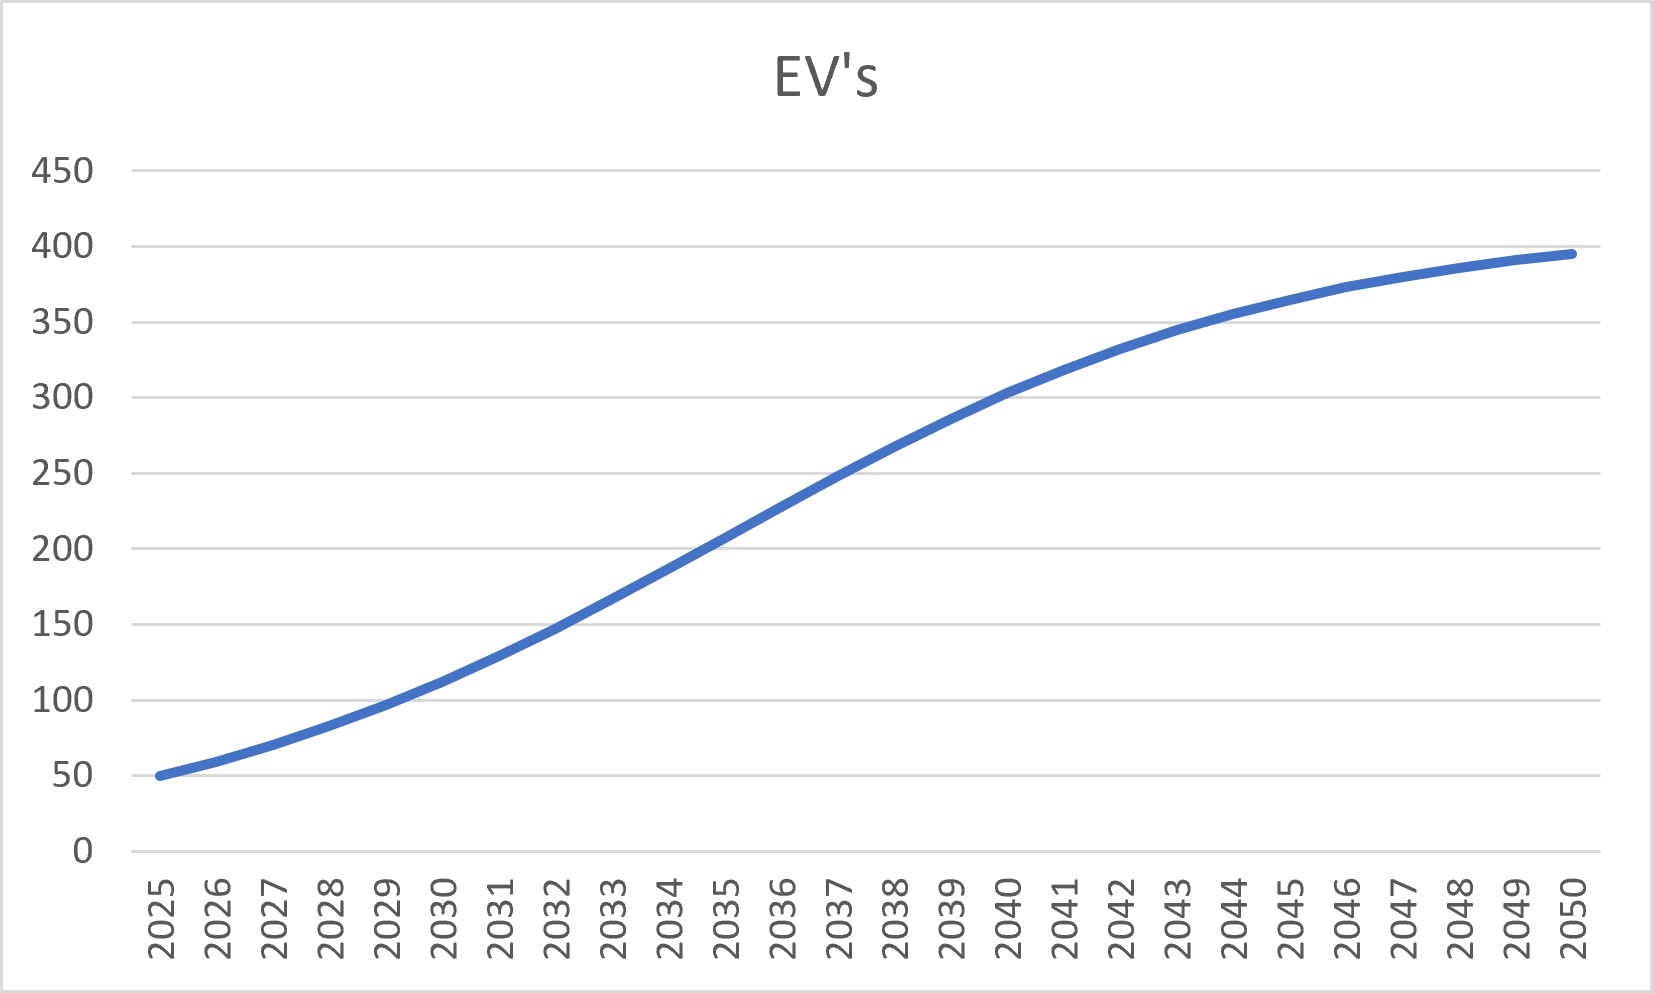
\includegraphics[width=0.8\linewidth]{figA1_ev_scurve.png}
  \caption{S-curve EV adoption for a random neighbourhood. The curve is similar for
  all neighbourhoods based on the total number of cars and the 2023 share of EVs.}
  \label{fig:ev-scurve}
\end{figure}
 
\begin{table}[htbp]
  \centering
  \caption{Network similarity and sizes for 20 random homeowners, used to verify
  the network algorithm.}
  \label{tab:network}
  \footnotesize
  \begin{tabular}{@{}r r r r r r@{}}
    \toprule
    \textbf{Homeowner} & \textbf{Owner attitude} & \textbf{Owner category} &
    \textbf{Owner network attitude} & \textbf{Network size} &
    \textbf{Same category \%}\\
    \midrule
    0  & 0.687 & 4 & 0.660 & 19 & 79\%\\
    1  & 0.923 & 2 & 0.877 & 22 & 86\%\\
    2  & 0.686 & 4 & 0.655 & 25 & 96\%\\
    3  & 0.933 & 2 & 0.882 & 29 & 90\%\\
    4  & 0.763 & 3 & 0.769 & 28 & 89\%\\
    5  & 0.665 & 4 & 0.655 & 23 & 91\%\\
    6  & 0.506 & 5 & 0.569 & 25 & 76\%\\
    7  & 0.829 & 3 & 0.777 & 24 & 83\%\\
    8  & 0.587 & 4 & 0.684 & 24 & 75\%\\
    9  & 0.480 & 5 & 0.518 & 24 & 92\%\\
    10 & 0.516 & 5 & 0.556 & 26 & 81\%\\
    11 & 0.211 & 6 & 0.343 & 25 & 96\%\\
    12 & 0.757 & 3 & 0.792 & 27 & 89\%\\
    13 & 0.687 & 4 & 0.642 & 30 & 83\%\\
    14 & 0.712 & 4 & 0.681 & 27 & 78\%\\
    15 & 0.984 & 2 & 0.882 & 26 & 89\%\\
    16 & 0.746 & 3 & 0.779 & 32 & 88\%\\
    17 & 0.683 & 4 & 0.664 & 31 & 71\%\\
    18 & 0.859 & 3 & 0.801 & 22 & 91\%\\
    19 & 0.861 & 3 & 0.794 & 24 & 92\%\\
    \bottomrule
  \end{tabular}
\end{table}
 
\section{Morris}
\begin{figure}[htbp]\centering
  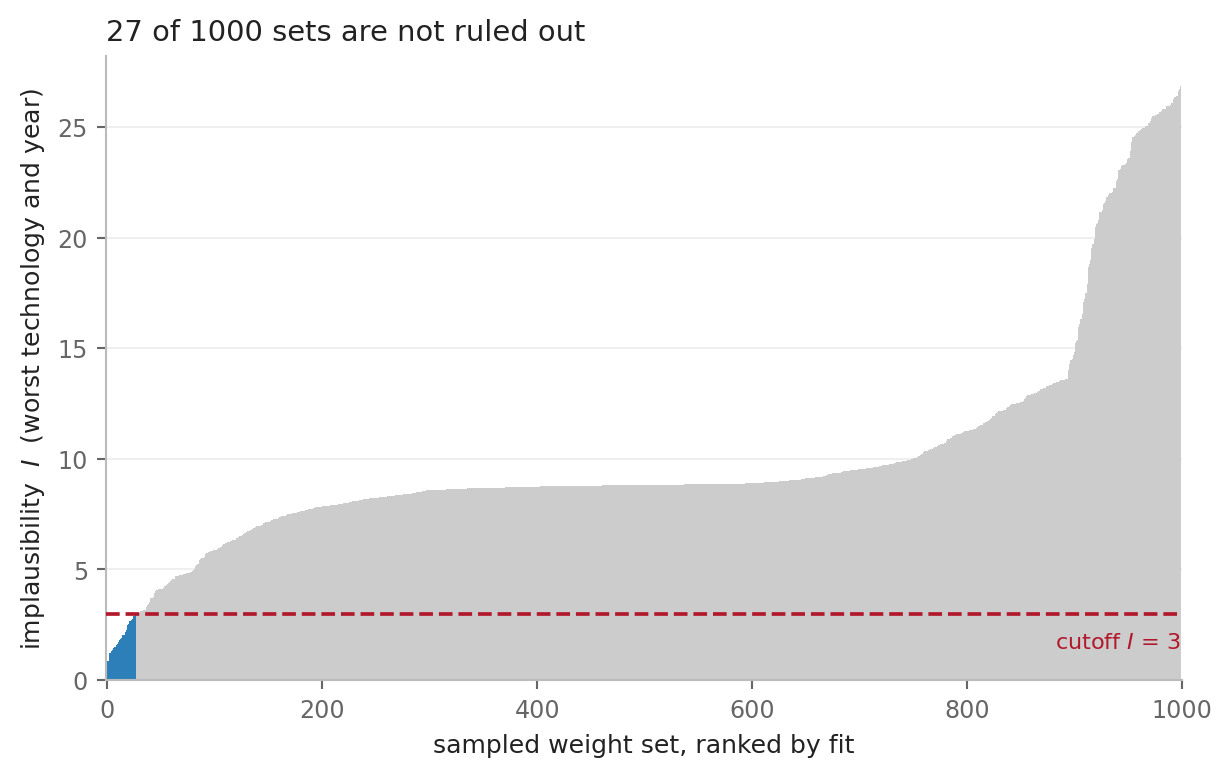
\includegraphics[width=\linewidth]{figures/fig_ensemble_fit.png}
  \caption{Fit of tested and retained ensemble}
  \label{fig:ensemble_fit}
\end{figure}


\section{Scenario pathways}
\label{app:scenariogrid}
Figure~\ref{fig:mix_all} gives the composition of the national heating stock over 2024--2050 for
every experiment in the design on common axes: the sixteen scenarios of the matrix as the median
over the retained weight ensemble, the two ends of the coupled energy-price bracket, and the loop
knock-outs against their intact reference, both at the central weights. The results sections draw
on subsets of this figure.

\begin{figure*}[htbp]\centering
  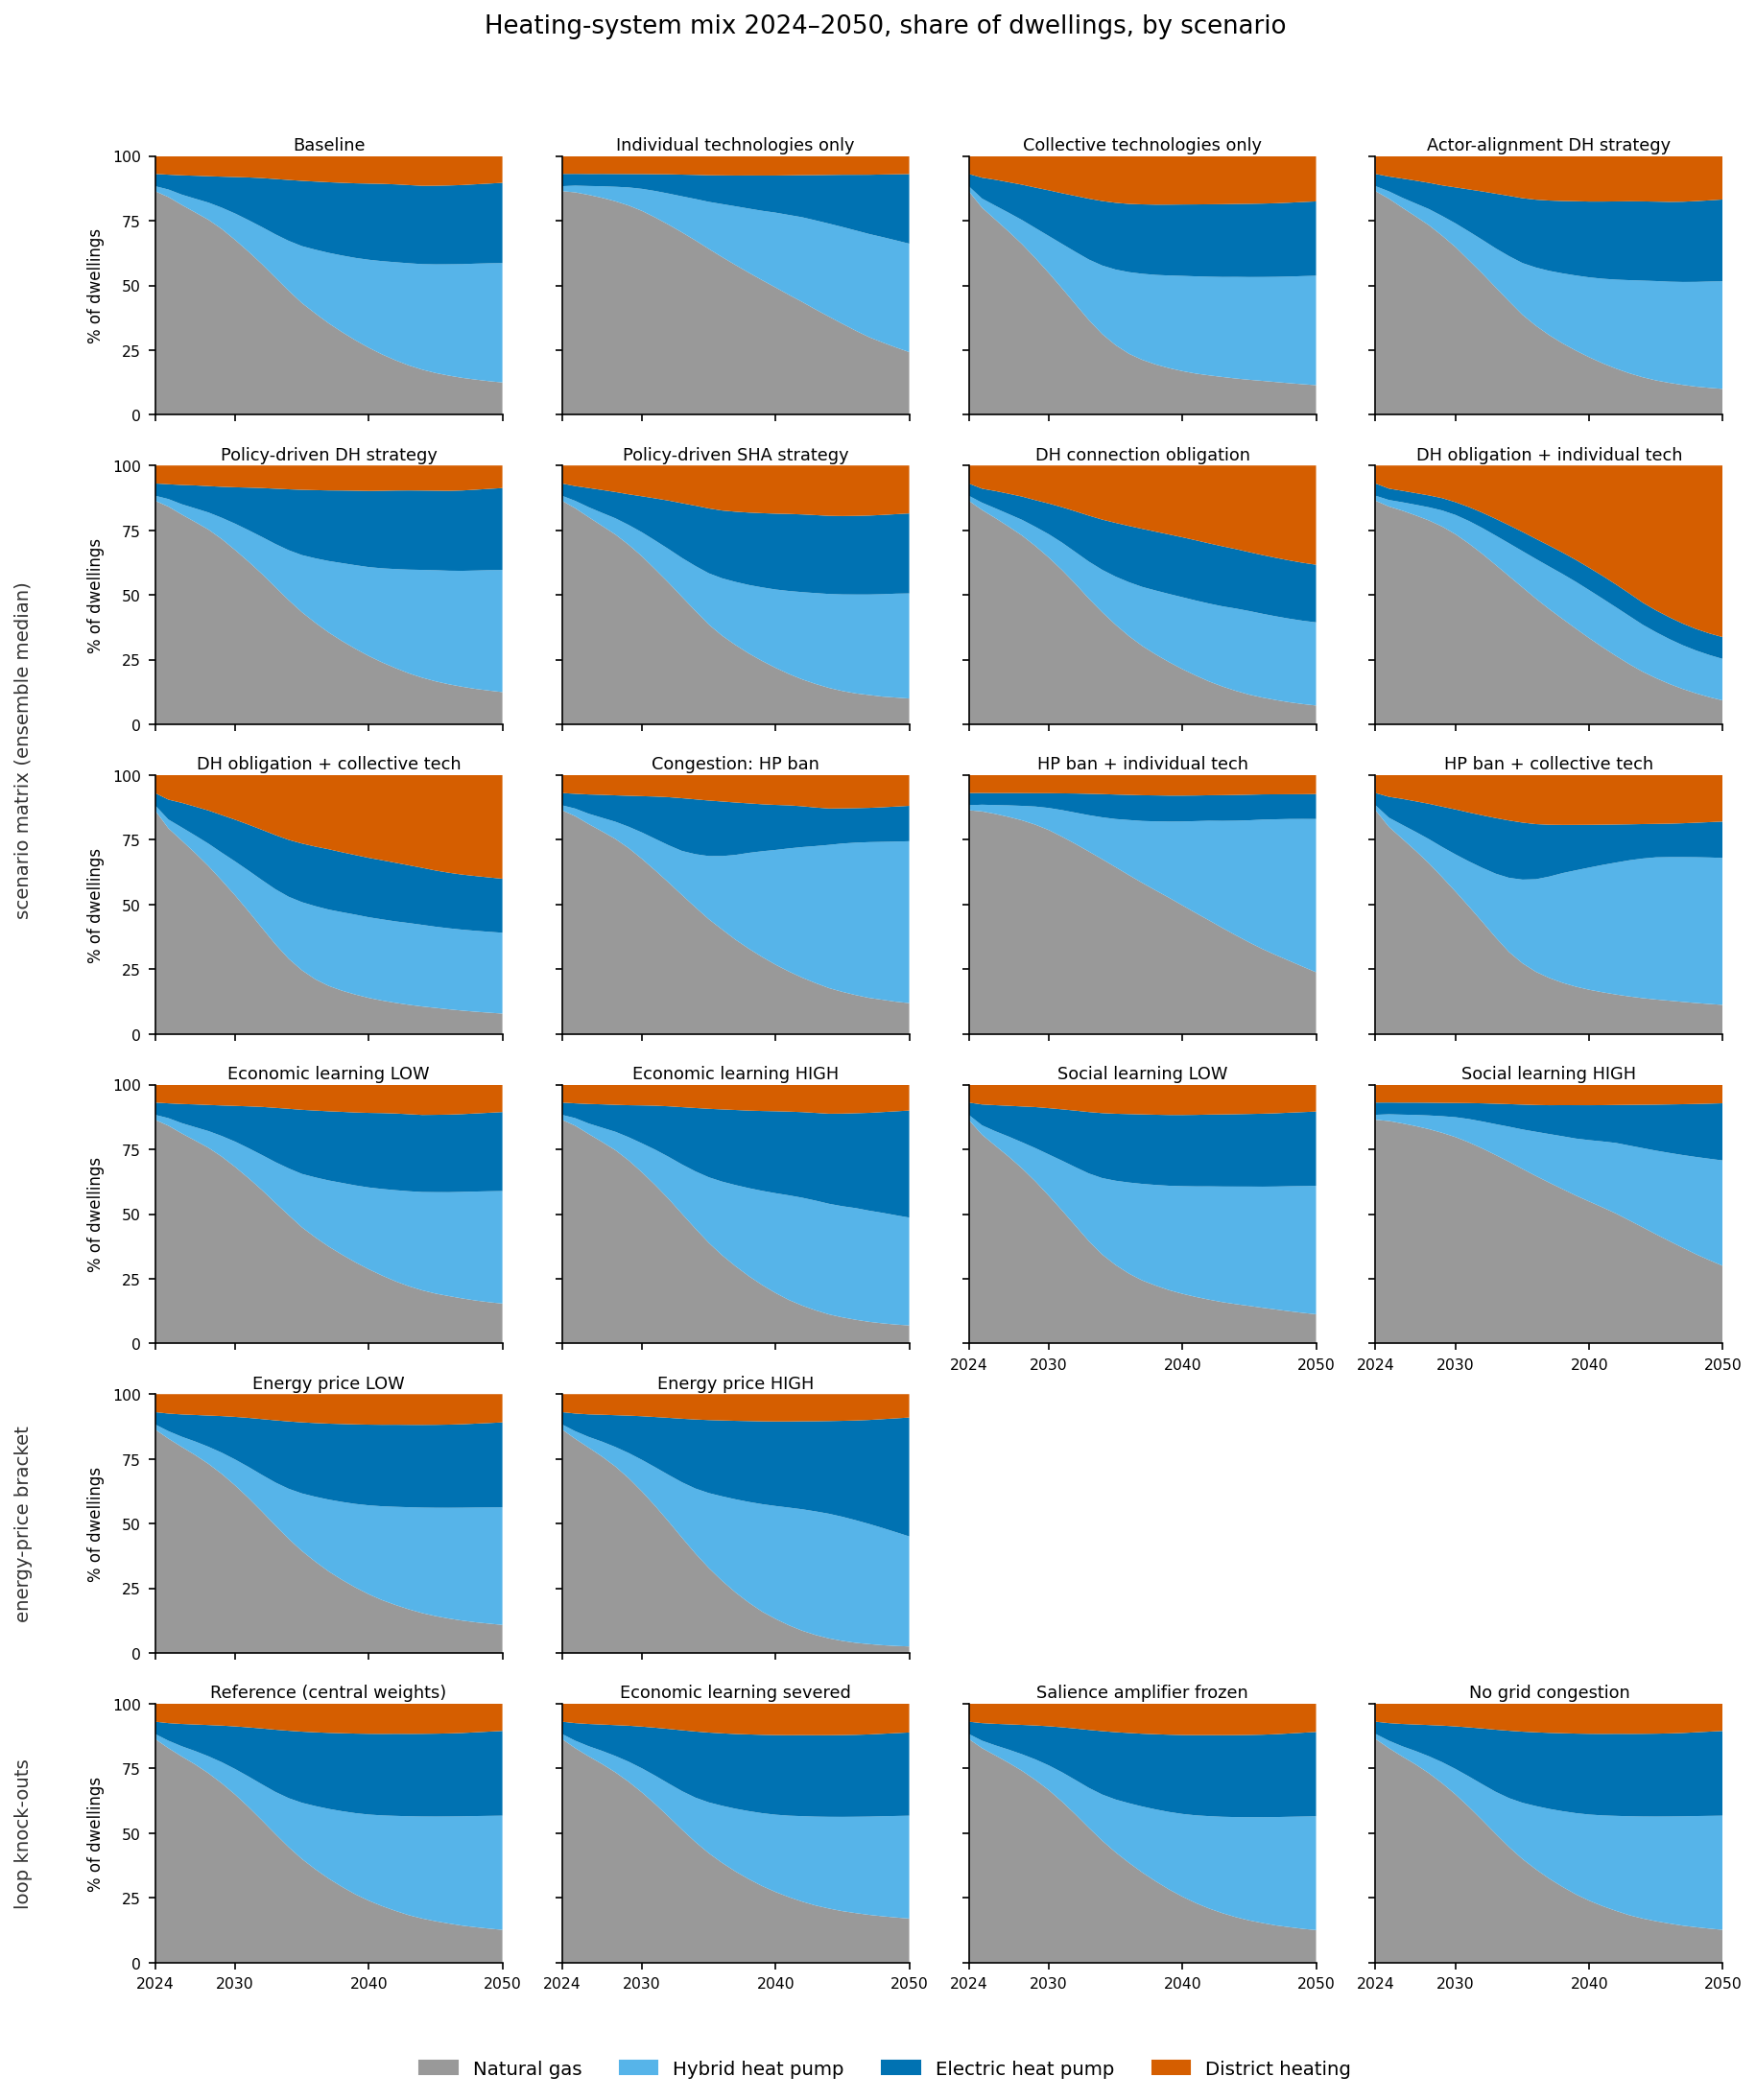
\includegraphics[width=\linewidth]{figures/fig_scenario_mix_all.png}
  \caption{National heating-system composition 2024--2050, share of dwellings, for every experiment
  in the analysis design.}
  \label{fig:mix_all}
\end{figure*}

\section{Reference dwellings}
\label{app:reference-dwellings}
 
% TODO: content for Appendix B (reference dwellings) was not present in the source.


\end{document}